\documentclass[12pt]{report}
\usepackage[margin=1.3in]{geometry}
\usepackage[T1]{fontenc}
\usepackage[utf8]{inputenc}
\usepackage{color}
\usepackage{longtable}
\usepackage[table,xcdraw]{xcolor}
\usepackage{multirow}
\usepackage{listings}
\usepackage{xcolor}
\usepackage{hyperref}
\usepackage{graphicx}
\usepackage{caption}
\usepackage{subcaption}
\usepackage{comment}
\usepackage{tabularx}
\usepackage{adjustbox}
\usepackage{enumerate}
\usepackage[shortlabels]{enumitem}
\hypersetup{
    colorlinks=true,
    linktoc=all,     
    linkcolor=black,  
}
\usepackage{afterpage}
\newcommand\blankpage{%
    \null
    \thispagestyle{empty}%
    \newpage}
\renewcommand{\familydefault}{\sfdefault}

\title{%
  \textbf{e-Mobility for ALL} \\
  \large Design Document \\}

\author{Abbondanza Alessia - 995959\\
    Campo Marco Lorenzo - 103213\\
    De Luca Alessandro - 103542}
\date{December 2022}

\afterpage{\blankpage}
\begin{document}

\maketitle
\thispagestyle{empty}
\tableofcontents % Table of contents 
\thispagestyle{empty}
\cleardoublepage
\afterpage{\blankpage}

\chapter{Introduction}
\section{Purpose}
This is a design document (DD). The goal of this document is to provide a functional description of the e-MALL system previously presented in the Requirements Analysis and Specification Document (RASD). This document is intended for the development team and provides a detailed overview of the major components and their interaction.
In addition, the design decisions regarding the architecture are analyzed to provide developers with information about the architecture chosen (client-server) and the software and hardware components used to build the system, taking into account availability, reliability, performance, and security. Data management is also briefly discussed, in terms of the database chosen.
The design features contained in this document serve as a guide for the implementation, integration, and testing of the e-MALL system. The main features of this DD are as follows:
\begin{enumerate}
    \item High-level system architecture
    \item Main system components
    \item Interfaces provided by most important components
    \item Design patterns adopted
\end{enumerate}
The decision making process involved in the design of this distributed system is explained in depth throughout the document.

\section{Scope}
The full list of assumptions and requirements can be found in the associated RASD, but it can be summarized as follows: The e-MALL system should allow users to book, manage, and perform electric charges at registered stations and provide charging station operators with tools to manually manage these stations and interact with energy providers. The system also uses information provided by electric vehicles and stored data to provide users with an advanced feature for personalized charging plans.\\
As previously discussed in the RASD, e-MALL will be analyzed as two separate and communicating subsystems which both have specific properties. Both e-MALL CPMS and eMSP will share a few aspects of the architecture choices, but the implementation will differ heavily.\\
The system is designed for a very large number of users (as described in more detail in the RASD) distributed over a large region, and therefore needs to be distributed to provide fast and reliable access to the data for all connected users.

\section{Definitions, Acronyms}
\subsection{Definitions}
\begin{itemize}
    \item\textbf{e-MALL}: e-Mobility for All, software that will be analyzed in detail in this document
    \item\textbf{eMSP}: e-Mobility Service Providers, software to manage the interaction between users and charging stations
    \item\textbf{CPOs}: Charge Point Operators, who physically sets up the station and operates it. They interact with a CPMS.
    \item\textbf{CPMS}: Charge Point Management System, software used by CPOs to manage the charging station and the operations that take place there.
    \item\textbf{DSO}: Distribution System Operator, outside organization that provides the energy.\\
\end{itemize}

\subsection{Acronyms}
\begin{itemize}
    \item\textbf{API}: Application Programming Interface 
    \item\textbf{GPS}: Global Positioning System
    \item\textbf{MVC}: Model-View-Controller pattern
    \item\textbf{HTTP}: HyperText Transfer Protocol
    \item\textbf{SSL}: Secure Sockets Layer
    \item\textbf{JSON}: JavaScript Object Notation
    \item\textbf{EV}: Electric Vehicles
    \item\textbf{OCPI}: Open Charge Point Interface
    \item\textbf{OCPP}: Open Charge Point Protocol
\end{itemize}

\section{Revision History}
    \begin{itemize}
        \item Version 1.0 | 1.8.2023
    \end{itemize}

\section{Document Structure}
\begin{enumerate}
    \item\textbf{Introduction}: This chapter introduces the reader to the concept of the e-MALL system, highlighting the purpose and scope of DD. The section also includes the terms and acronyms used throughout the report.
    \item\textbf{Architectural Design}: This chapter contains the architectural design decisions made during the development of the e-MALL system with respect to the software and hardware elements used. The Runtime View and Component Interfaces sections contain the main functions provided by the interfaces and the processes that use them.
    \item\textbf{User Interface Design}: This chapter presents some mockups of the user interface in special sections, multiple for each user type if required.
    \item\textbf{Requirements Traceability}: This chapter presents the mapping between the requirements defined in the RASD and the architectural elements chosen.
    \item\textbf{Implementation, Integration and Testing}: This chapter contains plans for implementing, integrating, and testing the various components of the system presented in this document.
    \item\textbf{Effort Spent}: Provides an overview of the effort spent by each group member in order to complete the DD.
\end{enumerate}

\chapter{Architectural Design}
\section{Overview: High-level components and interaction}
The e-MALL System adopts a three-tiered client-server architecture, applied differently for each subsystem.\newline
The decision to use a three-tier architecture was made to separate the business logic of the system from the data. The data itself could more usefully be used for other applications and modules in the future, and decoupling facilitates this.\newline
The system has also been designed to be updated and integrated with multiple functions to follow the trend towards new energy sources and technologies. Therefore, a decoupled architecture can help in this regard.\newline
Additionally, it provides one more layer of security, as all data access passes through the middle layer.\\
The architecture consists in the following layers:

\begin{enumerate}[L1:]
        \item\textbf{Presentation layer}: This layer is responsible for the interaction with the user. It contains all the interfaces needed for users and CPOs to communicate with the logic of the system;
        \item\textbf{Application layer}: This layer processes the business logic for the application and acts as a bridge between the other two layers;
        \item\textbf{Data layer}: This layer is a Database Management System (DBMS) and provides access to the application data. It provides an interface to the Application Layer and stores all relevant data for
        both user presentation and correct functioning of the back end system.
\end{enumerate}

\subsection{High-Level Component View}
\bigskip

The architecture described above is implemented using three-tier hardware, with each tier associated with a layer. The following image summarizes the chosen architectural style.
\bigskip 

\begin{figure}[ht]
    \centering
    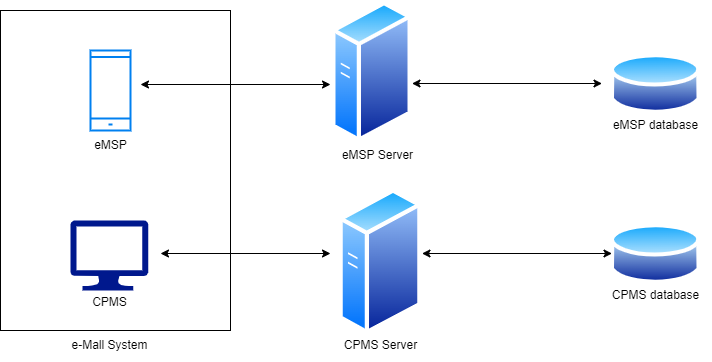
\includegraphics[width =\textwidth]{assets/high_level_system.drawio.png}
    \caption{Three-tiered hardware architecture}
    \label{fig:my_label0}
\end{figure}

\newpage
\bigskip
\begin{enumerate}[T1:] 
    \item\textbf{Client}: Provides an interface for interacting with the system. It can be provided via a desktop (CPMS) or a smartphone (eMSP);
    \item\textbf{Application server}: Processes requests provided from the client and provides business logic;
    \item\textbf{Data Source}: Contains both the DBMS and any external data sources. Different data sources are queried from eMSP or CPMS servers.
\end{enumerate}

\noindent The devices used by different users (desktop or smartphones) correspond to the client level of the hardware architecture. All devices are connected to the correspondent application server. The latter represents the server layer of the architecture and provides interaction with DBMS and (if demanded) external APIs.

\section{Component View}
\subsection{Component Diagram}
The component diagram below describes the organization and wiring of the internal structure of the application server, which contains the business logic of the software, and the interaction between the various components.\\
 \begin{figure}[htbp]
\hspace*{-2.5cm}   
    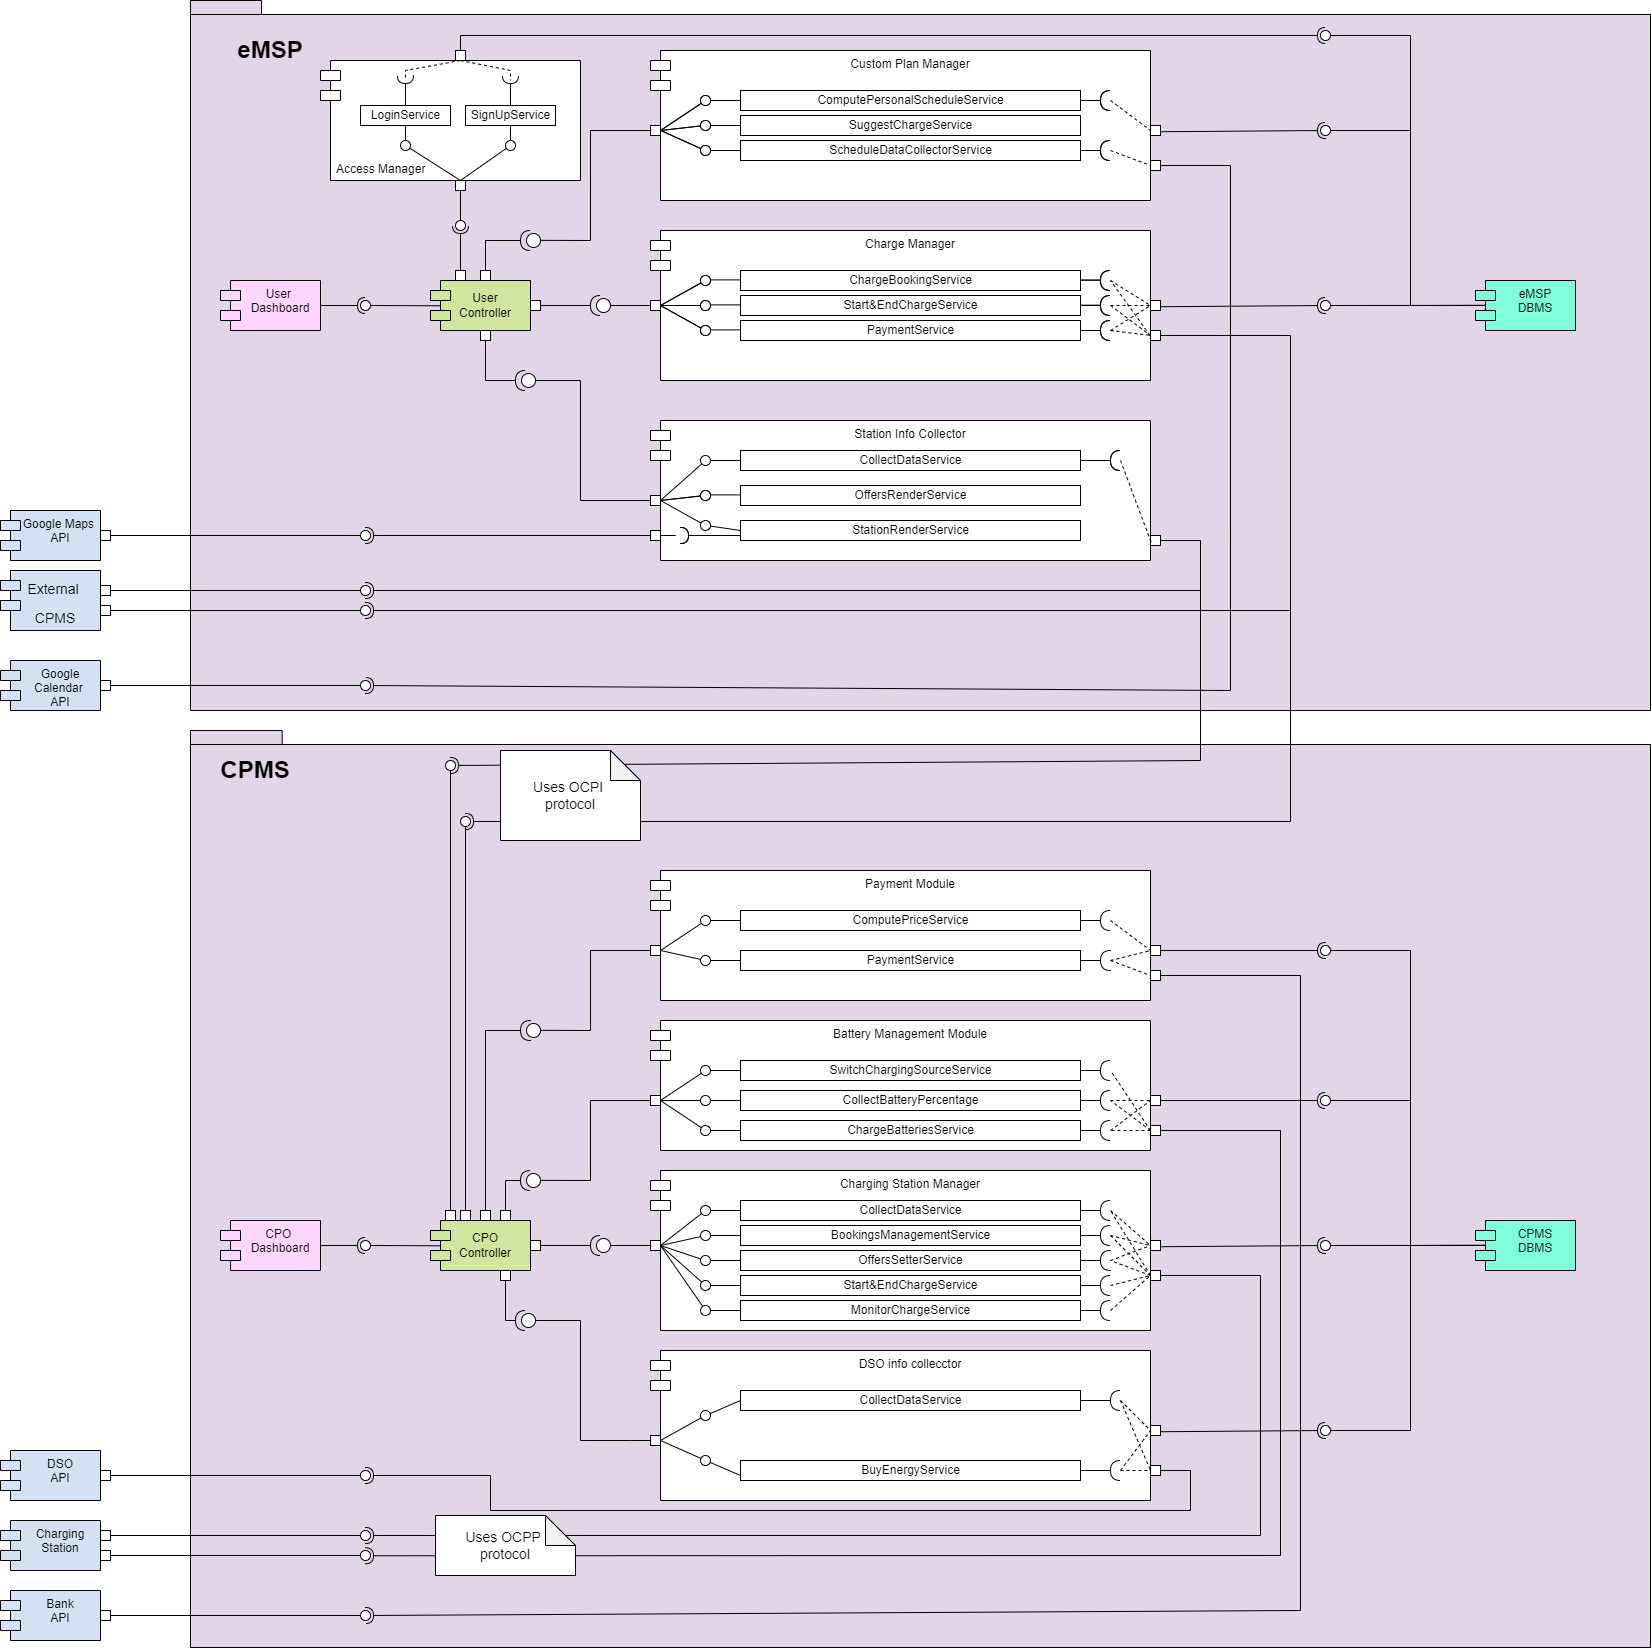
\includegraphics[width = 1.3\textwidth]{assets/component_complete.png}
    \caption{Component diagram of the whole e-MALL system}
    \label{fig:my_label9}
\end{figure}\\
\clearpage


\subsubsection{eMSP Component Diagram}
\begin{figure}[h]
    \hspace*{-2.5cm} 
    \centering
    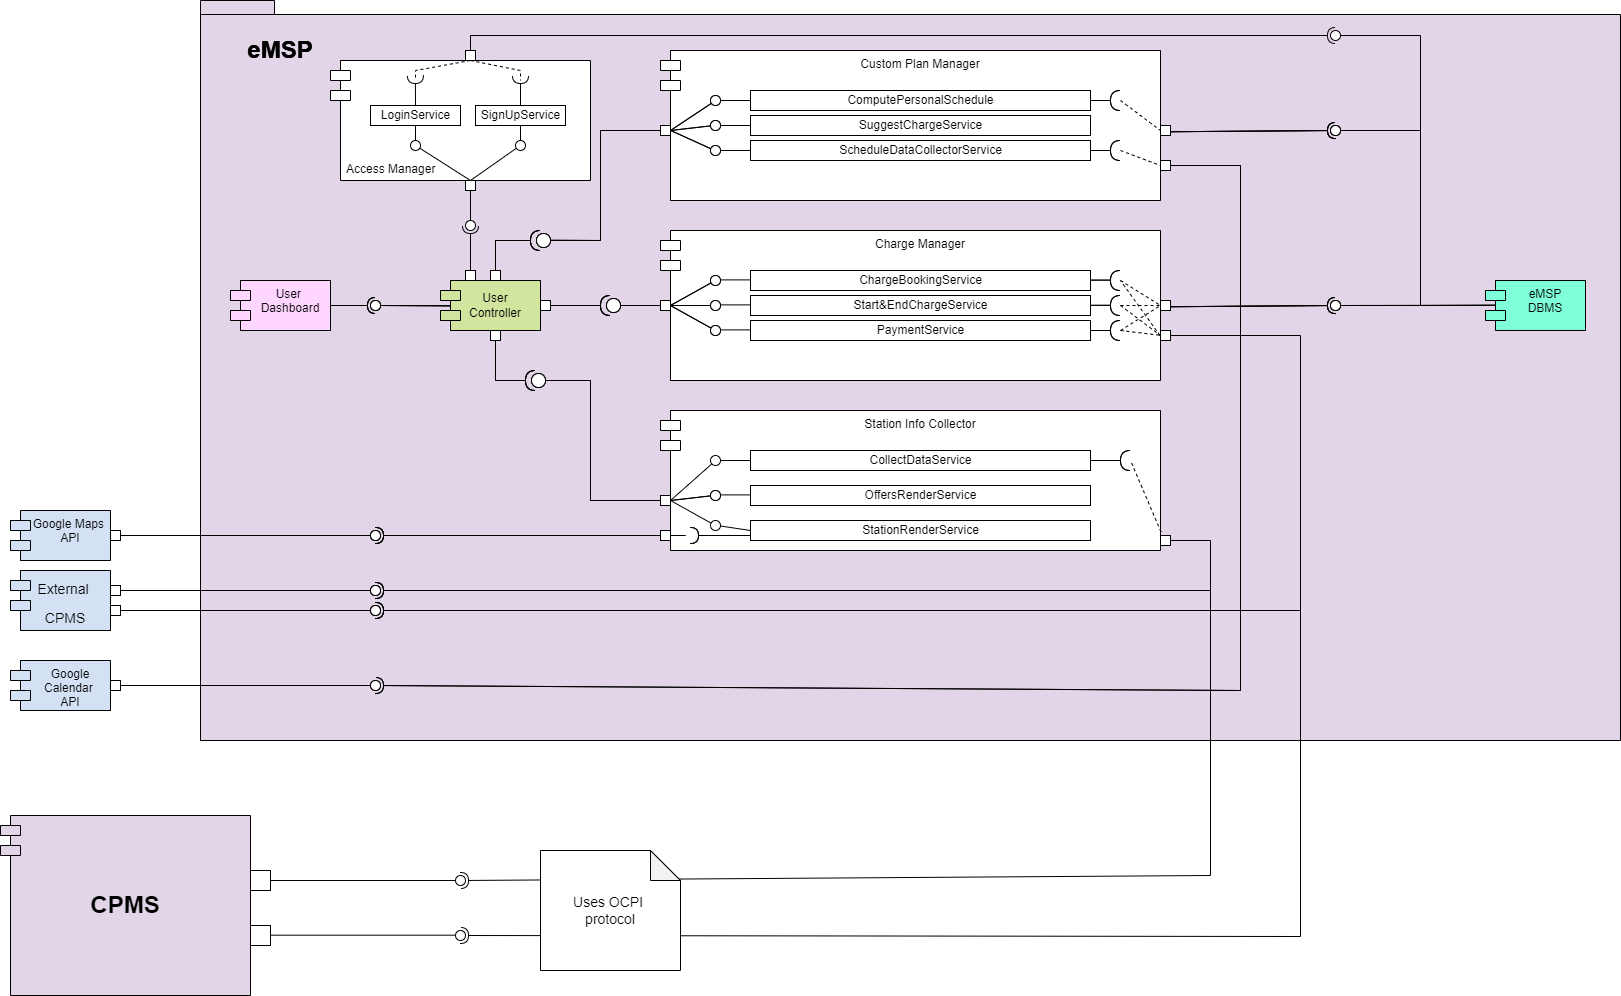
\includegraphics[width = 1.3\textwidth]{assets/component_emsp.png}
    \caption{Component diagram of the e-MALL eMSP}
    \label{fig:my_label7}
\end{figure}

\begin{itemize}
    \item[C1.]\textbf{Google Maps API}: APIs used by the e-MALL eMSP to get the rendering of a specific geographical area
    \item [C2.] \textbf{Google Calendar API}: APIs used by the e-MALL eMSP to get the user's personal schedule 
    \item [C3.] \textbf{External CPMS}: Contact interface provided by external CPMS. e-MALL eMSP can communicate with them in order to provide better coverage 
    \item [C4.] \textbf{User Dashboard}: Component that allows users to interact with the eMALL system, provided by a GUI
    \item [C5.] \textbf {User Controller}: Component that redirects the user's input to the correct module depending on the user's actions
    \item [C6.] \textbf {Access Manager}: Component that manages sign up and sign in actions
    \item [C7.] \textbf{eMSP DBMS}: Database management system that supports the user side of the system. This component collects data to provide both a more personalized experience and less communication with external components when they are not needed.
    \item [C8.] \textbf{Custom Plan Manager}: This component is responsible for creating and managing the "smart schedule" advanced feature offered by the e-MALL system
        \begin{itemize}
            \item[C8.1]\textbf{ScheduleDataCollectorService}: Service responsible for querying the Google Calendar API to obtain the data about the user's personal schedule
            \item [C8.2]\textbf{SuggestChargeService}: Service Responsible for notifying the user when a recharge is needed (a custom plan is being followed, a new offer has been published, the estimated battery level is low)
            \item [C8.3]\textbf{ComputePersonalScheduleService}: Service that implements logic to adapt a charging schedule to the user's schedule. This service takes into account the usual routes and activities  repeated during the week in order to create the most feasible loading schedule possible
        \end{itemize}
    \item [C9] \textbf{Charge Manager}: This component is responsible of managing the charging process, from its booking to the payment
        \begin{itemize}
            \item [C9.1]\textbf{ChargeBookingService}: This service takes user input and notifies the CPMS that a charge is requested at a specific charging station for a specific charging location. After confirmation by the CPMS, it sends the result to the user, either "accepted" or "denied"
            \item [C9.2]\textbf{Start\&EndChargeService}: This service is responsible of actually starting and ending the charging process
            \item [C9.3]\textbf{PaymentService}: This service is responsible for providing the user with the price of a charge, receiving the payment information, and returning it to CPMS for processing
        \end{itemize}
    \item [C10] \textbf{Station Info Collector}: This component is responsible of showing the user all the information relative to the charging stations
        \begin{itemize}
            \item [C10.1]\textbf{CollectDataService}: This service connects to CPMS to get information about the external status of charging stations (availability of charging spots, time needed for a spot to become available, type of charging spots available, GPS coordinates of the charging station, available offers)
            \item [C10.2]\textbf{OffersRenderService}: This service is responsible of rendering all the available offers
            \item [C10.3]\textbf{StationRenderService}: This service interfaces with the Google Maps API and information collected by the CollectDataService to display maps of charging stations and provide the corresponding information
        \end{itemize}
\end{itemize}
\clearpage

\subsubsection{CPMS Component Diagram}
\begin{figure}[h]
    \hspace*{-2.5cm} 
    \centering
    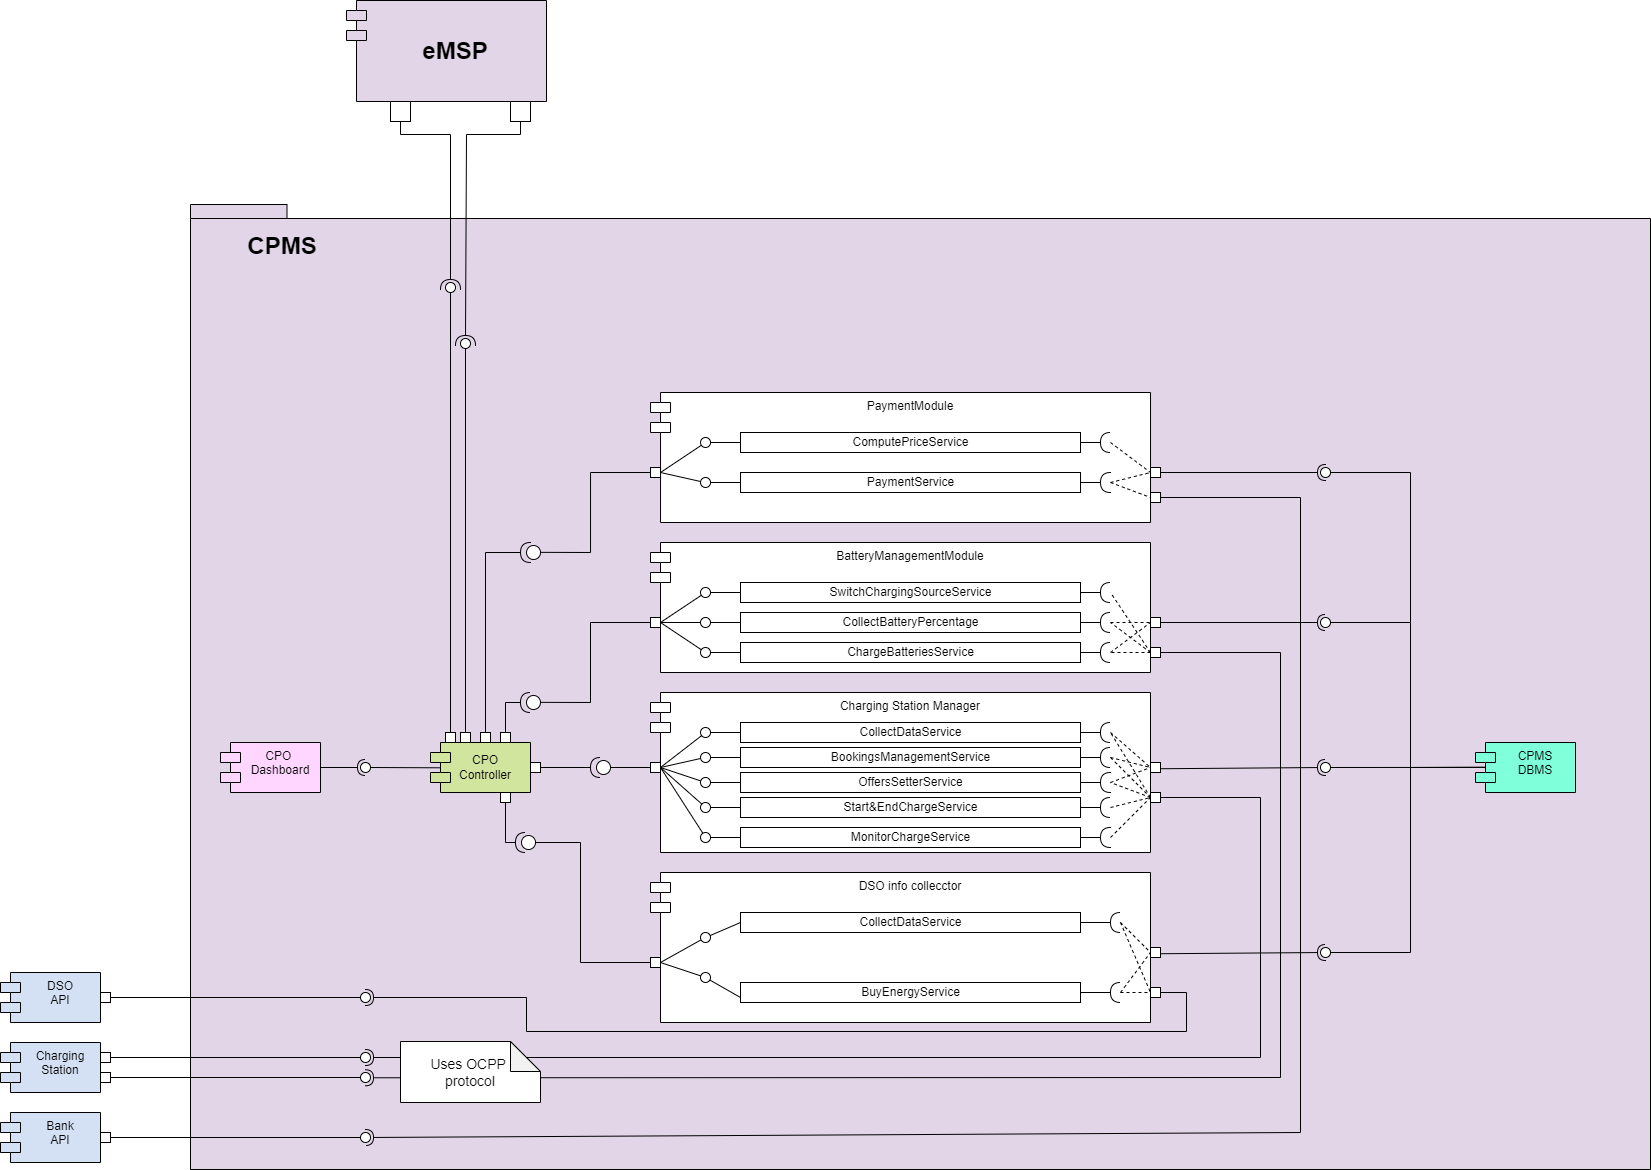
\includegraphics[width = 1.3\textwidth]{assets/component_cpms.png}
    \caption{Component diagram of the e-MALL CPMS}
    \label{fig:my_label8}
\end{figure}
\begin{itemize}
    \item [C1] \textbf{DSO API}:API to retrieve information about energy prices and purchase energy from a DSO
    \item [C2] \textbf{Charging Station}: interface of the charging station that sends information to the CPMS via certain communication protocols 
\item [C3] \textbf{Bank API}: API of the bank used to validate and execute payments 
\item [C4] \textbf{CPO Dashboard}: component that allows CPOs to interact with the CPMS and charging stations
\item [C5] \textbf{ CPO Controller}: controller used to route input from CPO and eMSP to the correct modules of the CPMS 
\item [C6] \textbf{ CPMS DBMS }: Database management system that supports the CPMS side of the system. This component collects data both for market analysis and diagnostics and to reduce communication with external components when not needed 
\item [C7] \textbf{payment module}: This module is responsible for handling all payment-related tasks
    \begin{itemize} 
        \item [C7.1]\textbf{ComputePriceService}: This service checks all information about an executed load (energy prices, type of load, time, amount of consumed energy) and calculates the final price of this load
        \item [C7.2]\textbf{PaymentService}: This service receives the user's payment information, sends it to the bank for verification, and responds to the user whether the transaction was approved or not
    \end{itemize}
\item [C8] \textbf{battery management module}: This module manages all functions related to the additional batteries present in a charging station
    \begin{itemize} 
        \item [C8.1]\textbf{SwitchChargingSourceService}: Service to switch the energy source from that provided by the DSO to that stored in the charging station batteries and vice versa 
        \item [C8.2]\textbf{CollectBatteryPercentage}: Service that monitors the remaining energy in the charging station batteries \item [C8.3]\textbf{ChargeBatteriesService}: Service used to initiate the charging of the batteries 
    \end{itemize} 
\item [C9]\textbf{Charging Station Manager }: Module that manages all functions related to the charging station 
    \begin{itemize} 
        \item [C9.1]\textbf{CollectDataService}: Service that collects all the information a charging station needs to know its internals (number of vehicles to be charged, amount of energy absorbed by each vehicle to be charged, time remaining until the end of the charging process)
        \item [C9.2]\textbf{BookingManagementService}: Service that manages bookings, validates booking requests (checks that there are no overlaps) and correctly classifies the specified time slot as occupied for the user who booked it, otherwise responds with an "input not valid" message 
        \item [C9.3]\textbf{OffersSetterService}: Service that allows CPO to post an offer 
        \item [C9.4]\textbf{Start\&EndChargeService}: Service that takes user input to startand stop a charging process and forwards it to the correct charging location 
        \item [C9.5]\textbf{MonitorChargeService}: Service that monitors the charging status of a vehicle connected to a time slot 
    \end{itemize} 
\item [C10] \textbf{DSO Info Collector}: Moduele responsible for managing communication with DSOs \begin{itemize} 
    \item [C10.1]\textbf{CollectDataService}: Service that connects to a DSO to collect information about the energy such as price, means of production, and availability 
    \item [C10.2]\textbf{BuyEnergyService}: Service that contacts a DSO to purchase energy from it 
    \end{itemize}
\end{itemize}

\subsection{More on communication protocols}
As described in the RASD, the system implements the three main communication protocols: OCPP, OCPI, DIN/ISO. These are the \emph{state of the art} in electrical charges.\newline

\subsubsection{Future assumpions}
For simplicity, all messages exchanged between eMSP and CPMS are sent in the format required by OCPI and all messages exchanged between CPMS and EV charger are sent in the format required by OCPP, even if this isn't specified.
Also the message exchange between EV charger and CPMS isn't shown in all provided diagrams, because the OCPP communication protocol is very straightforward and the notation can easily become redundant and cumbersome.

\subsubsection{OCPI Protocol}
The OCPI implementation used by e-MALL is version 2.2, and the implemented architecture is \emph{Hub and Peer-to-Peer}. Not all Platforms will only communicate via a Hub. There might be different reasons for Platforms to still have peer-to-peer
connections or the Hub might not yet support new functionalities. This also allows for better routing and control over the OCPI message exchange.


\begin{figure*}[b]
    %\hspace*{-2.5cm} 
    \centering
    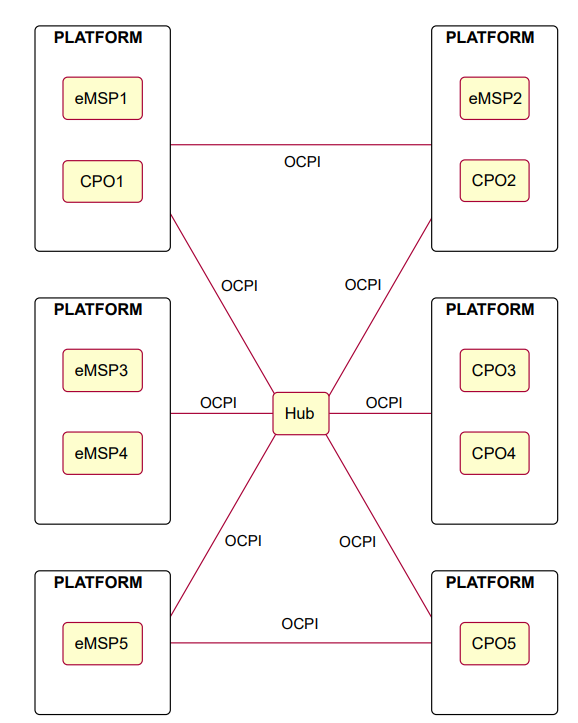
\includegraphics[width =0.7\textwidth]{assets/Platforms connected via a Hub and directly topology example.png}
    \caption{Platforms connected via a Hub and directly topology example}
    \label{fig:my_label99}
\end{figure*}
\clearpage

\noindent Message routing functionality also makes it possible to support platforms that host multiple roles. Many of the stakeholders are not just CPO or eMSP but both. Some parties have a platform where they host services for other CPOs/eMSPs. Some providers are CPO themselves and provide CPO services to others, while other providers (themselves) do not play a CPO or other role in the EV charging landscape, but provide services to CPOs/eMSPs.\newline
For this reason, having a very versatile infrastructure can benefit the system, especially considering future functionalities that may need to be implemented.\\

\noindent The OCPI protocol is based on HTTP, with SSL and server-side token-based authentication, and uses the JSON format. It follows a RESTful architecture for web services where possible.\\


\subsubsection{OCPP Protocol}
e-MALL has implemented OCPP 1.6J version, which means using JSON over WebSocket.\newline
The OCPP, Open Charge Point Protocol, is the standardized framework for communication between EV chargers, Electric Vehicle Supply Equipment (EVSE), and back end software. It sends information to the back end regarding start/stop/status messages for charging sessions, EVSE reservations, and firmware updates.\\

\noindent The protocol was chosen against competitors because it is free to use and hardware-agnostic, making the e-MALL CPMS service's target as big as it can possibly be. Also, OCPP is the most common communication protocol implemented in the EV charging landscape, so frequent patches and new functionalities are to be expected.\newline
The last major update concerns security. In version 1.6, the connection between the electric vehicle supply equipment and the backend of the network required a VPN to encrypt the entire communication channel. Now, data packets are encrypted at the protocol level, and no third party is needed for a secure connection. All big steps towards a secure and functional electrified infrastructure.\newline

\noindent The version chosen is the 1.6J which is the most commonly used one. In addition to the features mentioned above, 1.6 enables smart charging, the ability for the Network Operator to set restrictions like power level or time limits on an individual charger, TriggerMessages, allowing the Network to query information from the charger, and Authorized Local Lists, to determine who is allowed to charge on each unit.



\clearpage
\subsection{Additional Specification}
To ensure that the application provides high reliability and availability, the Application Server, which is the server tier, is replicated. Replication provides redundancy in case both the software and hardware fail. Load balancers are available to balance requests and prevent system overload, so that users can have the best possible experience depending on their location.

\begin{figure}[ht]
    \centering
    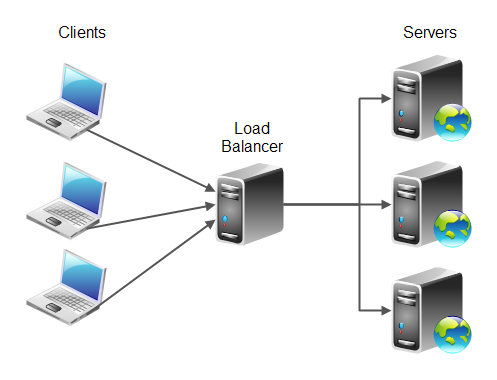
\includegraphics[width = 0.9\textwidth]{assets/load_balancers_and_replication.png}
    \caption{\emph{Load Balancer} and \emph{Replication} architecture}
    \label{fig:my_label1}
\end{figure}

\noindent To ensure more reliability and higher performance, the use of caches is essential as it will reduces the overall load on the servers.
The clients specified in the system architecture are thin clients, as they are designed to interact with the application server and do not provide any additional functionality without this connection. This allows the web application to verify the correctness of the compiled form by executing mobile code, while maintaining a lightweight manner required when dealing with low bandwidth.

\newpage
\section{Deployment view}

\begin{figure}[ht]
    \centering
    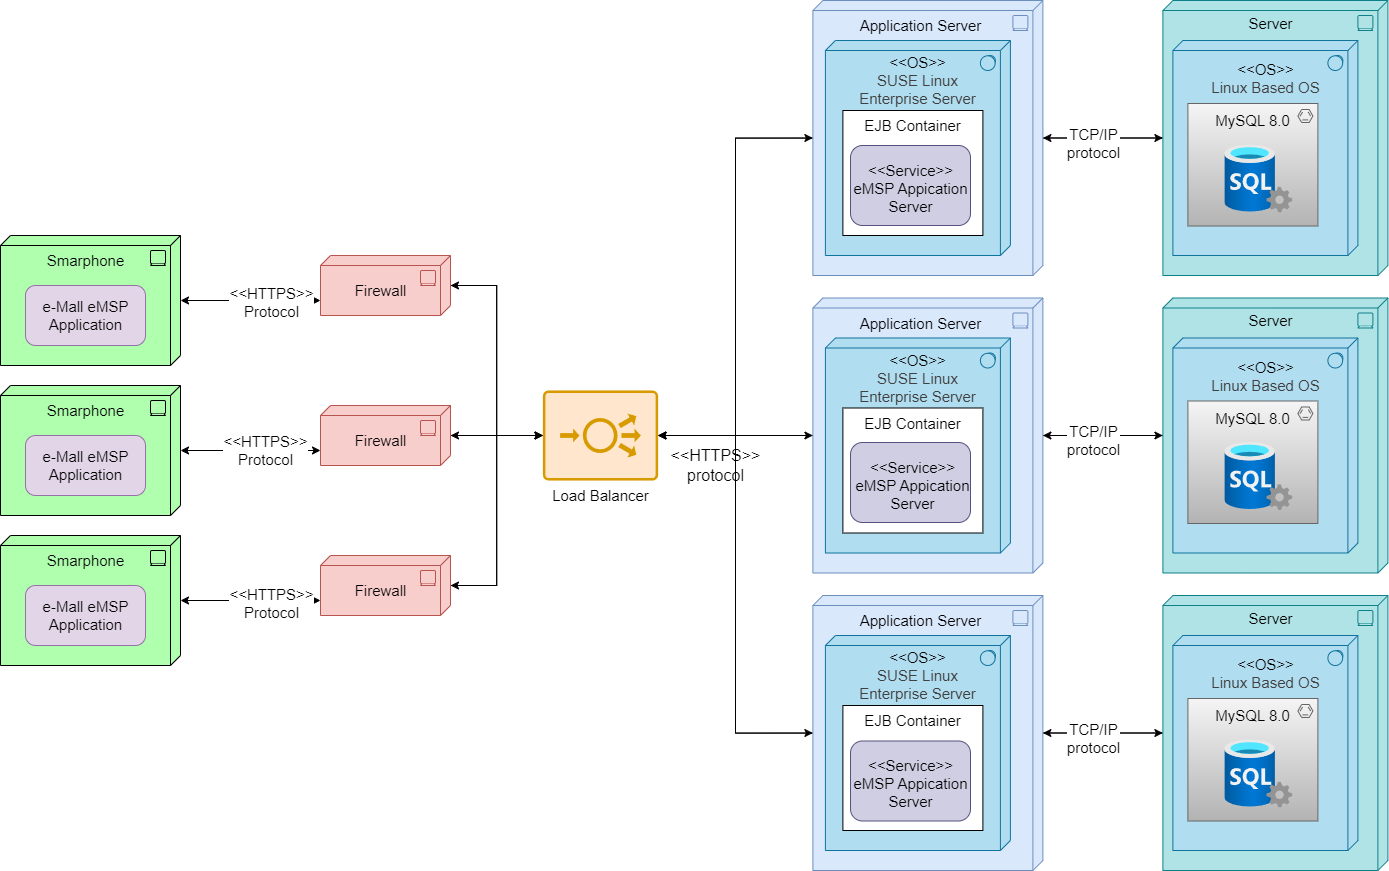
\includegraphics[width =1.1\textwidth]{assets/high_level_deployment_diagram_eMSP.drawio.png}
    \caption{Deployment diagram of the eMSP subsystem, three clients and \emph{server redundancy}}
    \label{fig:my_label2}
\end{figure}

\noindent Here are the main components of the system:

\begin{enumerate}[C1:] 
    \item\textbf{Smartphone}: User access device. It is used to connect to the Internet and perform various actions, such as: logging in/registering, booking and managing a charge, viewing the user's charge history, and custom plans. It can also display an overview of charging stations nearby or at a specific location. This is done by connecting to Google Maps' public APIs (which are not covered in this document);
    \item\textbf{Firewall}: Usual connection device in all domestic and enterprise networks. Prevents and controls inbound/outbound traffic;
    \item\textbf{Load Balancer}: It increases the reliability of the system by managing the distribution of the workload among the different servers;
    \item\textbf{Application Server}: Contains the business logic of the application and acts as \emph{middleware} placed between user and DBMS;
    \item\textbf{Database Management System}: It serves as an interface between the databases and the services run on the e-MALL application server.
\end{enumerate}

\begin{figure}[ht]
    \centering
    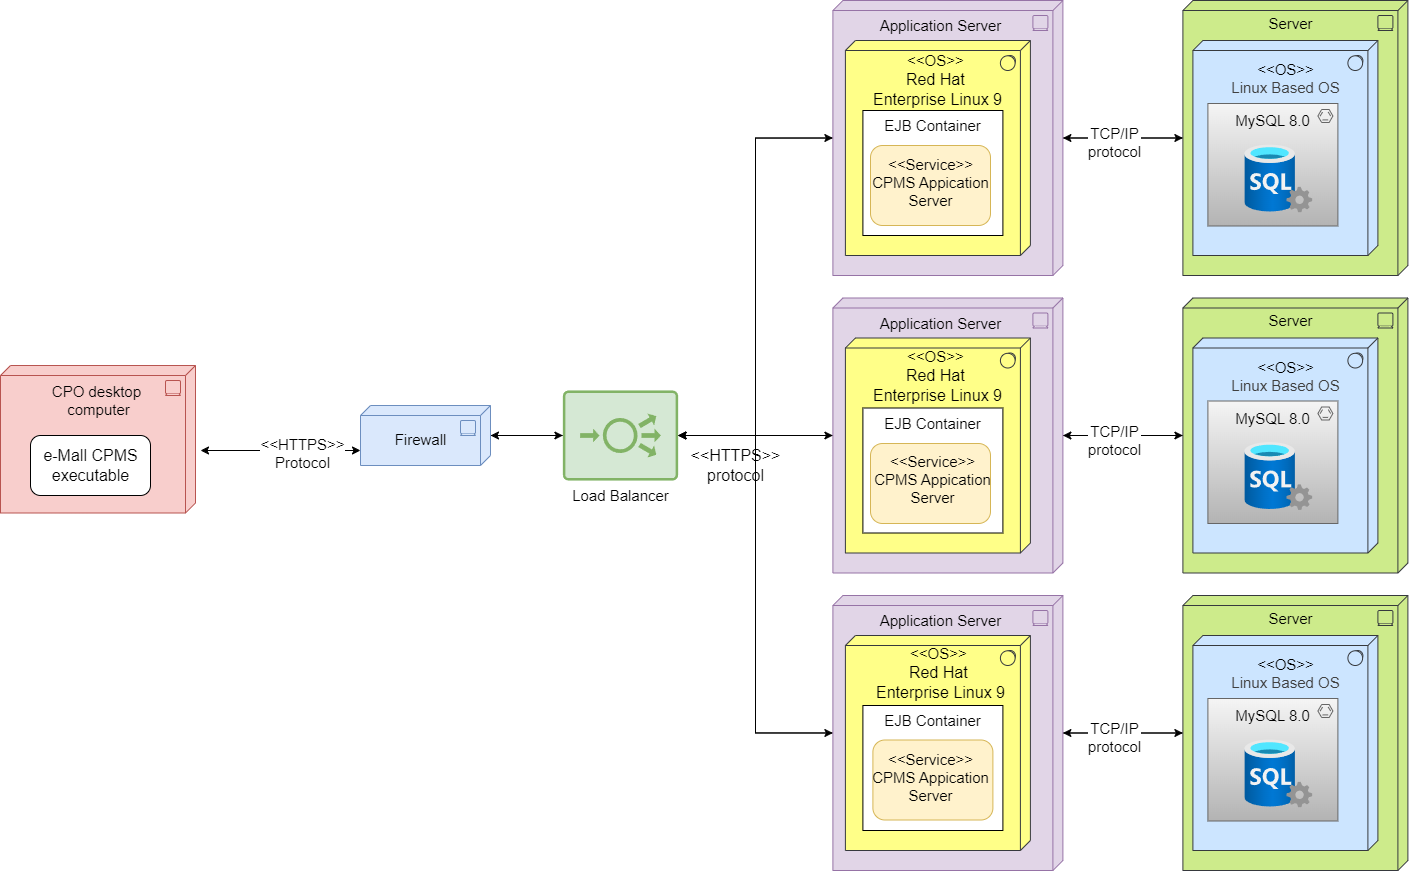
\includegraphics[width =1.1\textwidth]{assets/high_level_deployment_diagram_CPMS.drawio.png}
    \caption{Deployment diagram of the CPMS subsystem, one clients and \emph{server replication}}
    \label{fig:my_label3}
\end{figure}

\begin{enumerate}[C1:] 
    \item\textbf{Desktop computer}: Used by CPOs to connect to the Internet and gain control of the connected charging station. It is also the portal through which operators can advertise a new special offer and connect to DSOs for manual purchase of energy (through the APIs provided);
    \item\textbf{Firewall}: \emph{above mentioned};
    \item\textbf{Load Balancer}: \emph{above mentioned};
    \item\textbf{Application Server}: Contains the business logic of the application and acts as \emph{middleware} placed between CPOs and DBMS;
    \item\textbf{Database Management System}: It serves as an interface between the databases and the services run on the e-MALL application server.
\end{enumerate}

\subsection{More on deployment choices}

\begin{enumerate}
    \item SUSE Linux Enterprise Server (SLES) was chosen for the eMSP application server because of its versatility. It is designed for large workloads in big data centers, but also for single-server environments. Also, because it is subscription-based, it gives access to patches, fixes and security updates through the SLES customer portal, making future fixes and management easier, while keeping the system as reliable as possible.\\
    \item The DMBS of choice for implementation is MySQL 8 which can be easily scaled and follows a client-server architecture.\\
    \item Red Hat Enterprise Linux 9 was chosen for the CPMS application server because of its popularity, reliability and constant security patches, updates and support.
    \item A relational database was chosen because the data stored is by no means large or aggregated:
    \begin{itemize}
        \item[4.1]\textbf{eMSP data}:
            \begin{enumerate}[i.]
                \item Usercode and Password
                \item Bookings data: time frame, location, duration, prices, socket type, etc.
                \item Custom charging plans
                \item User's charging history
                \item Payment information:encrypted using the md5 encryption algorithm in order to guarantee all security measures
            \end{enumerate}
        \item[4.2]\textbf{CPMS data}:
            \begin{enumerate}[i.]
                \item Station's information
                \item Bookings data: user, time frame, socket type, etc.
            \end{enumerate}
    \end{itemize}
    Simple and predictable data types can provide good segmentation and storage, which facilitates maintenance and allows scalability.
\end{enumerate}


\newpage
\section{Runtime view}
In this section sequence diagrams will be used to describe the interaction between the most important components of the system, in such a way that developers can understand the functionalities to be implemented.\\
\begin{enumerate}[1.]
    \item\textbf{User books a charge}\\
    \\
    This sequence diagram represents the process of a user booking a charge on the e-Mall application. The request is sent to the User Controller, and then to the BookingManagementService. Then it is forwarded to the CPO controller, in particular to the ChargeBookService, that verifies it and sends back the messages of confirmation.
    \\
    \begin{figure}[ht]
    \centering
    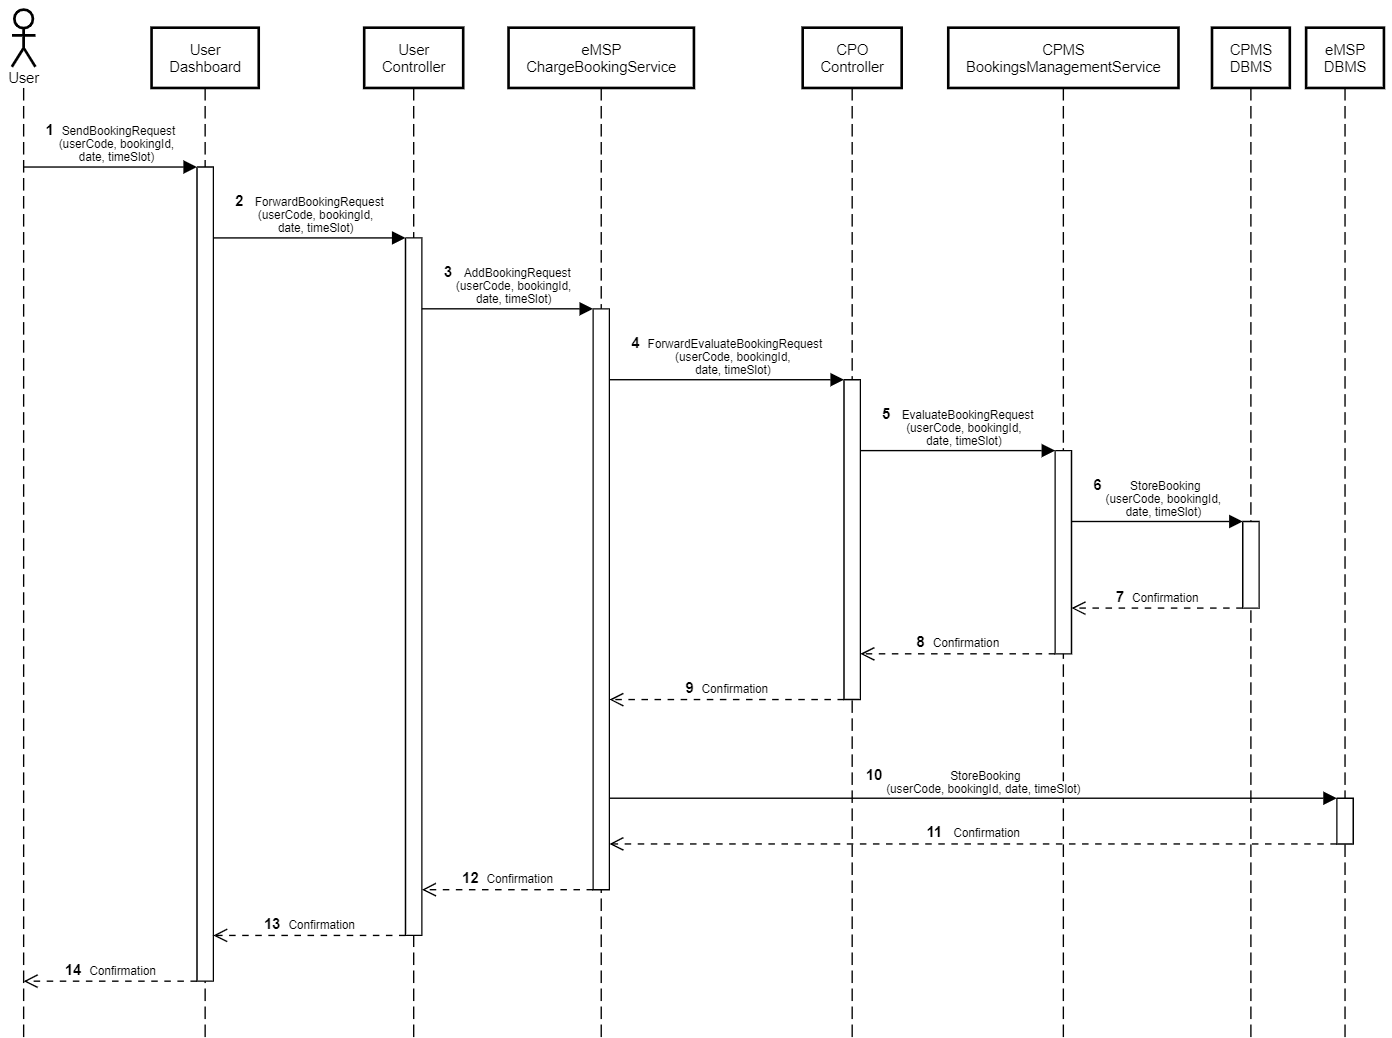
\includegraphics[width=\textwidth]{assets/sequencediagramBooking.png}
    \caption{Sequence diagram for a user booking a charge}
    \label{fig:my_label3423}
    \end{figure}

    \newpage
    \item\textbf{User starts a charge}\\
    \\
    The following sequence diagram displays the flow of a user starting a charge of the vehicle, communicating with the eMSP Start\&EndChargeService, which, in turn, communicates with the CPMS Start\&EndChargeService.
    \\
    \begin{figure}[ht]
    \centering
    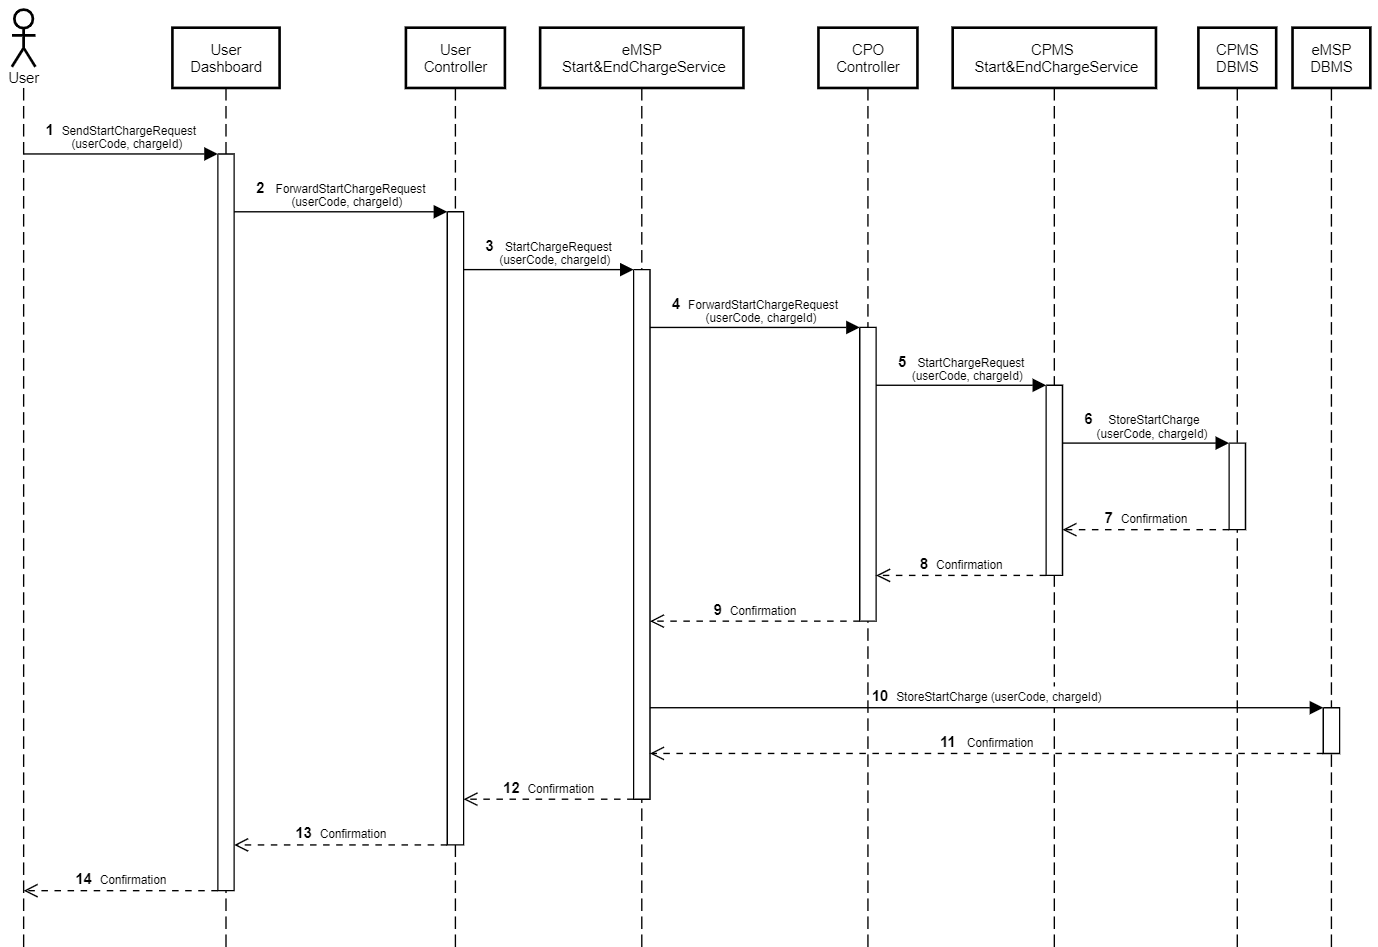
\includegraphics[width=\textwidth]{assets/sequencediagramCharge.png}
    \caption{Sequence diagram for a user starting a charge}
    \label{fig:my_label343453666}
    \end{figure}

\newpage

    \item\textbf{User pays for a charge}\\
    \\
    This sequence diagram shows the process of a user paying for a charge, sending the payment request to the eMSP PaymentService, which is forwarded to the CPMS PaymentService that asks for permission to the Bank API. If the payment is verified from the bank, the transaction is successful.
   \\
    \begin{figure}[ht]
    \centering
    \includegraphics[width=1.1\textwidth]{assets/sequenceDiagramPayment.png}
    \caption{Sequence diagram for a user paying for the charge}
    \label{fig:my_label34534534}
    \end{figure}
 

\newpage

    \item\textbf{CPO operator sets a special offer}\\
    \\
    This sequence diagram shows the flow generated when a CPO opertor tries to set a special offer for a specific charging station. The request is sent through the CPMS OfferSetterService, which adds it to the available offers.
    \\

     \begin{figure}[ht]
    \centering
    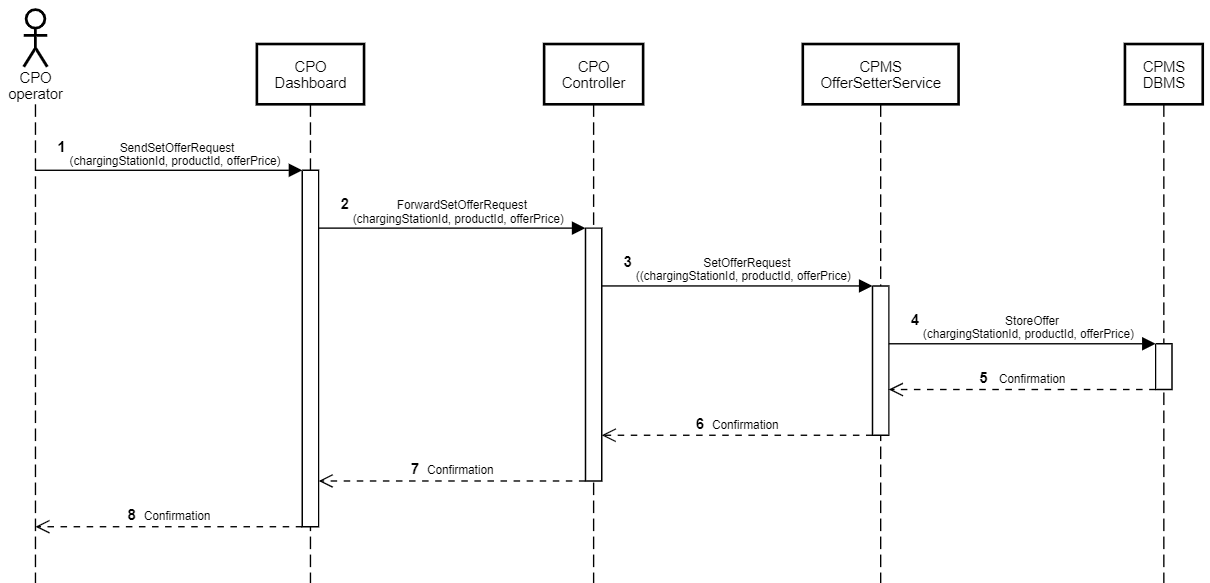
\includegraphics[width=\textwidth]{assets/sequencediagramOffer.png}
    \caption{Sequence diagram for a CPO operator setting a special offer}
    \label{fig:my_labelwerwer}
    \end{figure}
    
\newpage

    \item\textbf{User views custom daily plan}\\
    \\
    The following sequence diagram displays the process that happens when a user asks for the custom daily plan. The request of the plan is sent to the ComputePersonalScheduleService, which, in turn, asks for the calendar of the user to the GoogleCalendar API, and then proceeds to the creation of the plan, that is showed to the user.\\


    \begin{figure}[ht]
    \centering
    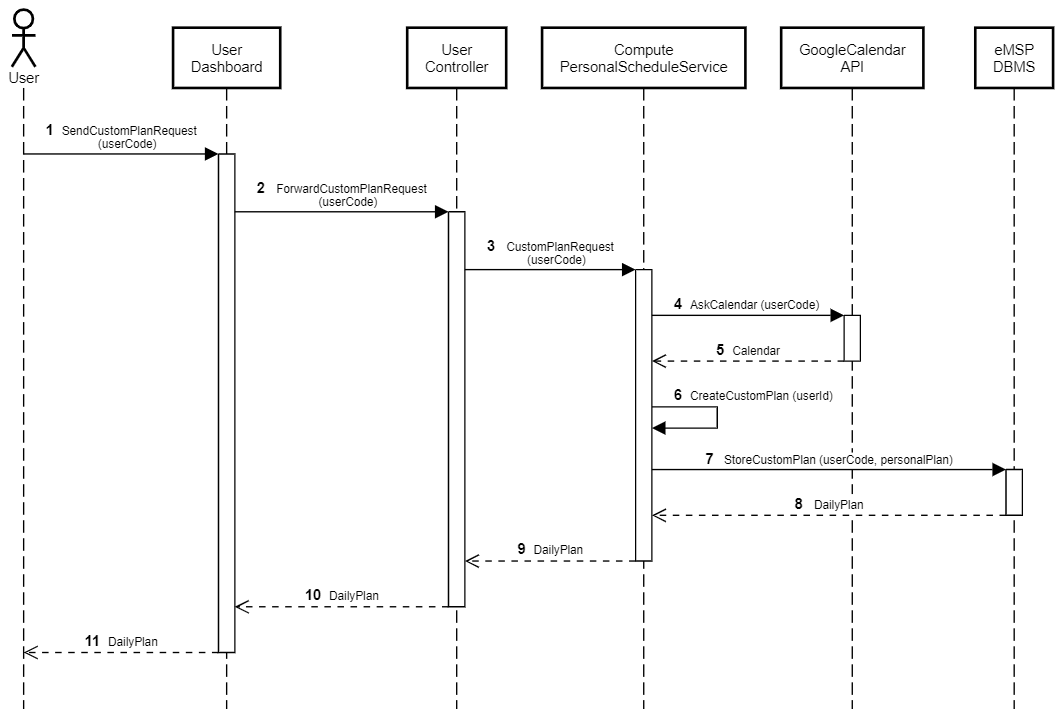
\includegraphics[width=\textwidth]{assets/sequencediagramPlan.png}
    \caption{Sequence diagram for a user asking for the daily plan}
    \label{fig:my_label6}
    \end{figure}


    \newpage


    \item\textbf{CPO operator buys energy from a DSO}\\
    \\
    This sequence diagram shows the flow of a CPO operator buying a certain quantity of energy from a DSO, forwarding the request  to the CPMS BuyEnergyService, that contacts the DSO API to buy the energy. \\


    \begin{figure}[ht]
    \centering
    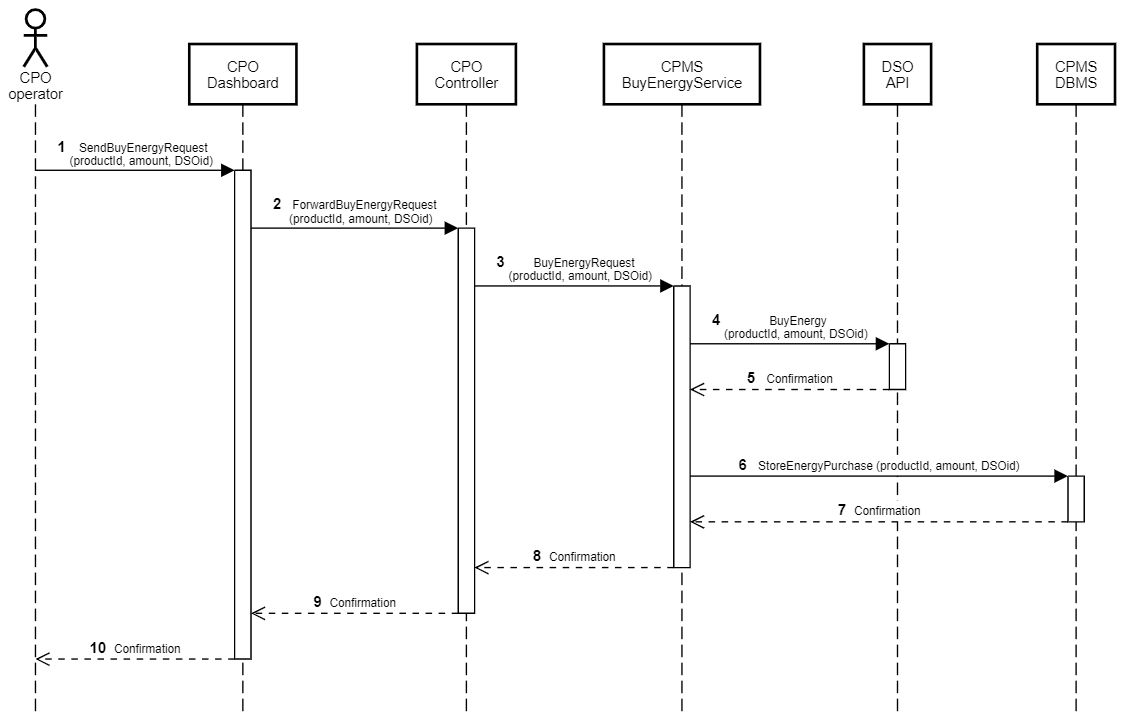
\includegraphics[width=\textwidth]{assets/sequencediagramBuyenergy.png}
    \caption{Sequence diagram for a CPO operator acquiring energy from a DSO}
    \label{fig:my_label6675}
    \end{figure}

    \newpage
    
\end{enumerate}




\section{Component interfaces}
The following diagram shows the main methods of the components interfaces of the system. These methods are useful to give a general idea of the functionalities that each part should provide.\\
\begin{figure}[h]
    \hspace*{-2cm}
    \centering
    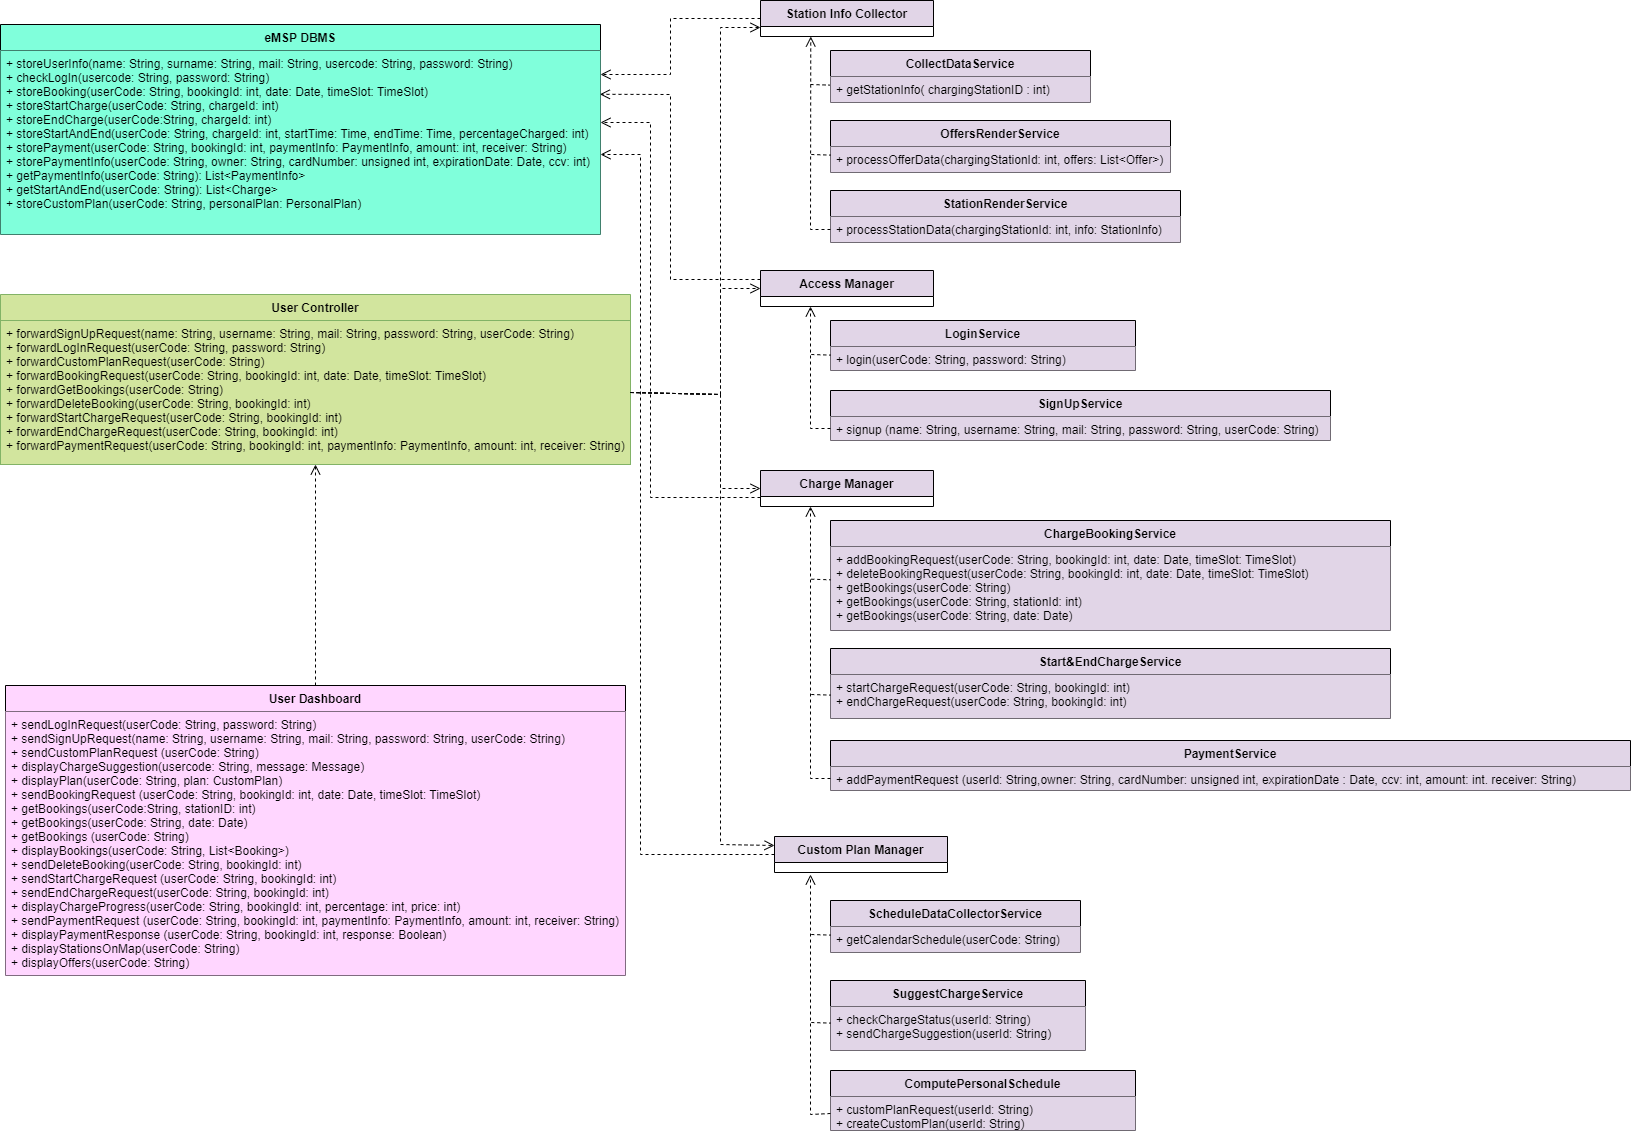
\includegraphics[width = 1.3\textwidth]{assets/interface_emsp.png}
    \caption{eEMSP interfaces}

\end{figure}
\begin{figure}[h]
    \hspace*{-2cm}
    \centering
    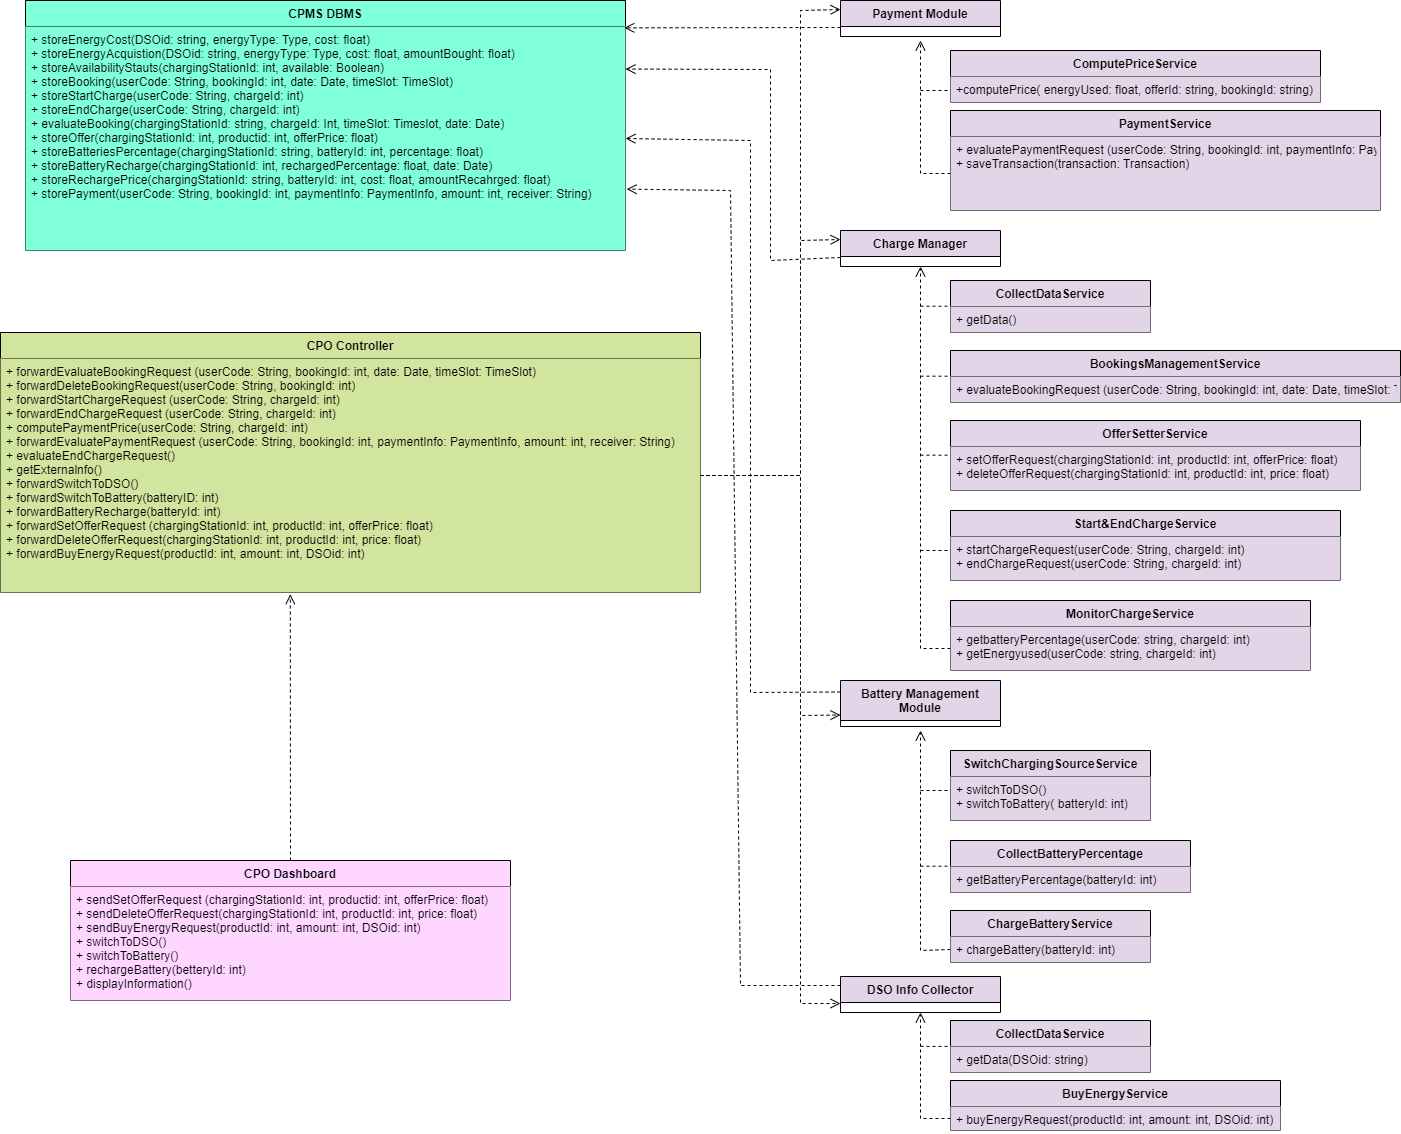
\includegraphics[width = 1.3\textwidth]{assets/interface_cpms.png}
    \caption{CPMS interfaces}
\end{figure}
\clearpage

\section{Selected architectural styles and patterns}

\bigskip
\textbf{Client-Server architecture}\\
As mentioned in the architecture overview, a three-tier client/server architecture was chosen. This architectural style offers the advantage that all data is stored in a central location, namely the server, which greatly facilitates the development and maintenance of the application.\\
Client/server architectures restrict communication to defined interfaces between clients and servers. This restriction simplifies communication between clients and servers, reducing potential vulnerabilities in the architecture. Another advantage of this architectural style is the distinction between three tiers. The three-tier client/server architecture decouples the logic of the data and the logic of the presentation, which increases the security and protection of the data, as well as making the development of the system easier.\\
Smartphones and computers are also capable of storing small amounts of data in cache memory. Cache memory is used to reduce the number of requests made by the client to the server.\\

\bigskip
\noindent\textbf{HTTPS protocol}\\
HyperText Transfer Protocol Secure (HTTPS) is the selected protocol for data communication between the components of the system. HTTPS encrypts the data to protect privacy and increase the security of the system to prevent Man In The Middle (MITM) attacks and phishing campaigns.
The data transmitted in the network is in a JSON format which is a less verbose language, making communication and debugging easy to manage.\\

\bigskip
\noindent\textbf{Model-View-Controller pattern}\\
MVC (Model-View-Controller) is a pattern in software design commonly used to implement user interfaces, data, and control logic. It emphasizes the separation between the business logic of the software and the display. This "separation of concerns" provides better division of labor and improved maintenance.\\
Another important aspect of the MVC pattern is the independence of the three parts, each one can be developed and later integrated with the others.\\
The three parts of the MVC software design pattern can be described as follows:
\begin{itemize}
    \item\textbf{Model}: Manages data and business logic. Includes DBs, DBMSs, data structures, and services for storing, managing, and processing user inputs.
    \item\textbf{View}: Takes care of the layout and display of the system. Any state-changing action is provided to the rest of the system through the GUIs (Views).
    \item\textbf{Controller}: Relays commands to the model and view parts. Acts as an intermediary between the view and the model, translating the input provided by the user and the model's responses.
\end{itemize}

\begin{figure}[ht]
    \centering
    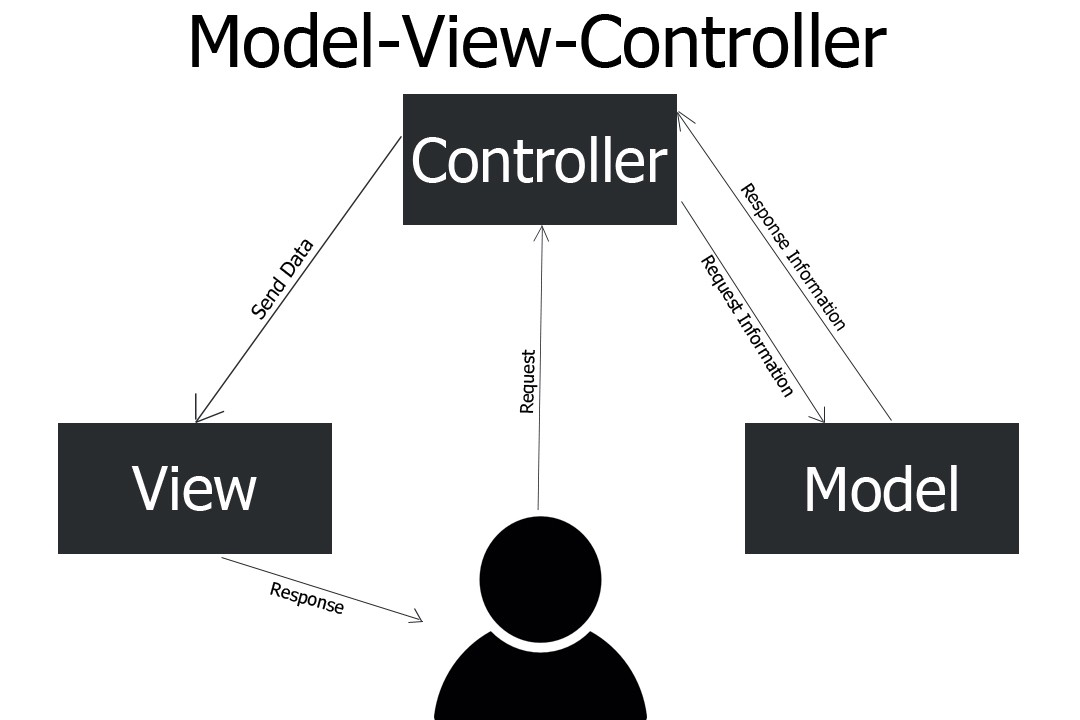
\includegraphics[width=0.6\textwidth]{assets/model-view-controller.jpg}
    \caption{\emph{Model-View-Controller} conceptual schema}
    \label{fig:my_label4}
\end{figure}
\clearpage

\chapter{User Interface Design}
This section focuses on the user interfaces that will be to interact with the system. In particular the most imporant features will be displayed.
\section{Client User Interface}
The images below are a mockup of what to expect by the client-side eMALL application. The features shown are the login interface, the charging station search, the booking, offers, and charge interface and the smart plan feature interface.

\begin{figure}[h]
        \centering
        \begin{subfigure}{0.49\textwidth}
        \centering
        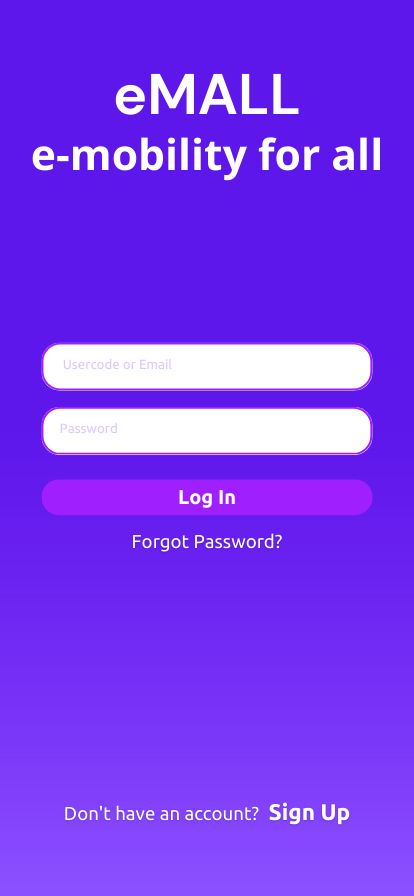
\includegraphics[width = 0.7\textwidth]{assets/ui1.png}
        \end{subfigure}
        \begin{subfigure}{0.49\textwidth}
        \centering
        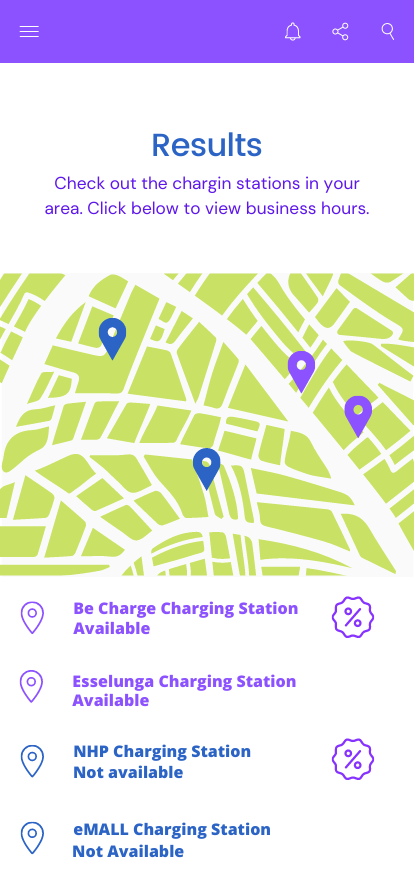
\includegraphics[width = 0.7\textwidth]{assets/ui2.png}
        \end{subfigure}
         \begin{subfigure}{0.49\textwidth}
        \centering
        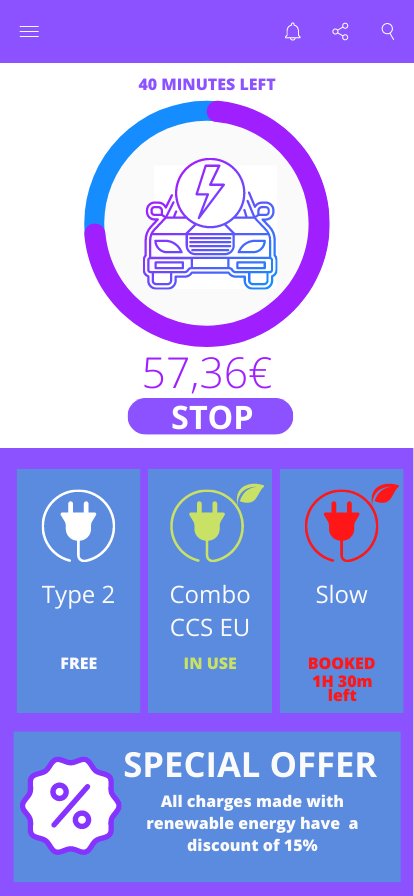
\includegraphics[width = 0.7\textwidth]{assets/ui3.png}
        \end{subfigure}
        \begin{subfigure}{0.49\textwidth}
        \centering
        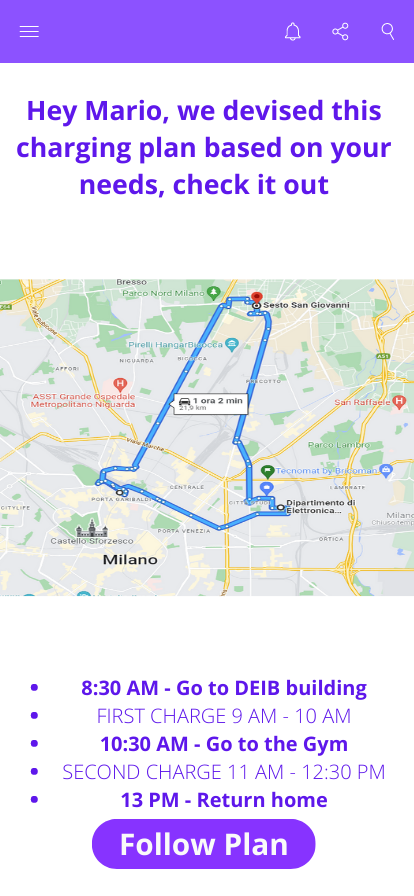
\includegraphics[width = 0.7\textwidth]{assets/ui4.png}
        \end{subfigure}
        \caption{User interfaces}
\end{figure}

\clearpage
\section{CPO User Interface}
The figure below shows a mockup of the CPO Dashboard of the CPMS.\\

\begin{figure}[h]
        \centering
        \begin{subfigure}{0.49\textwidth}
        \centering
        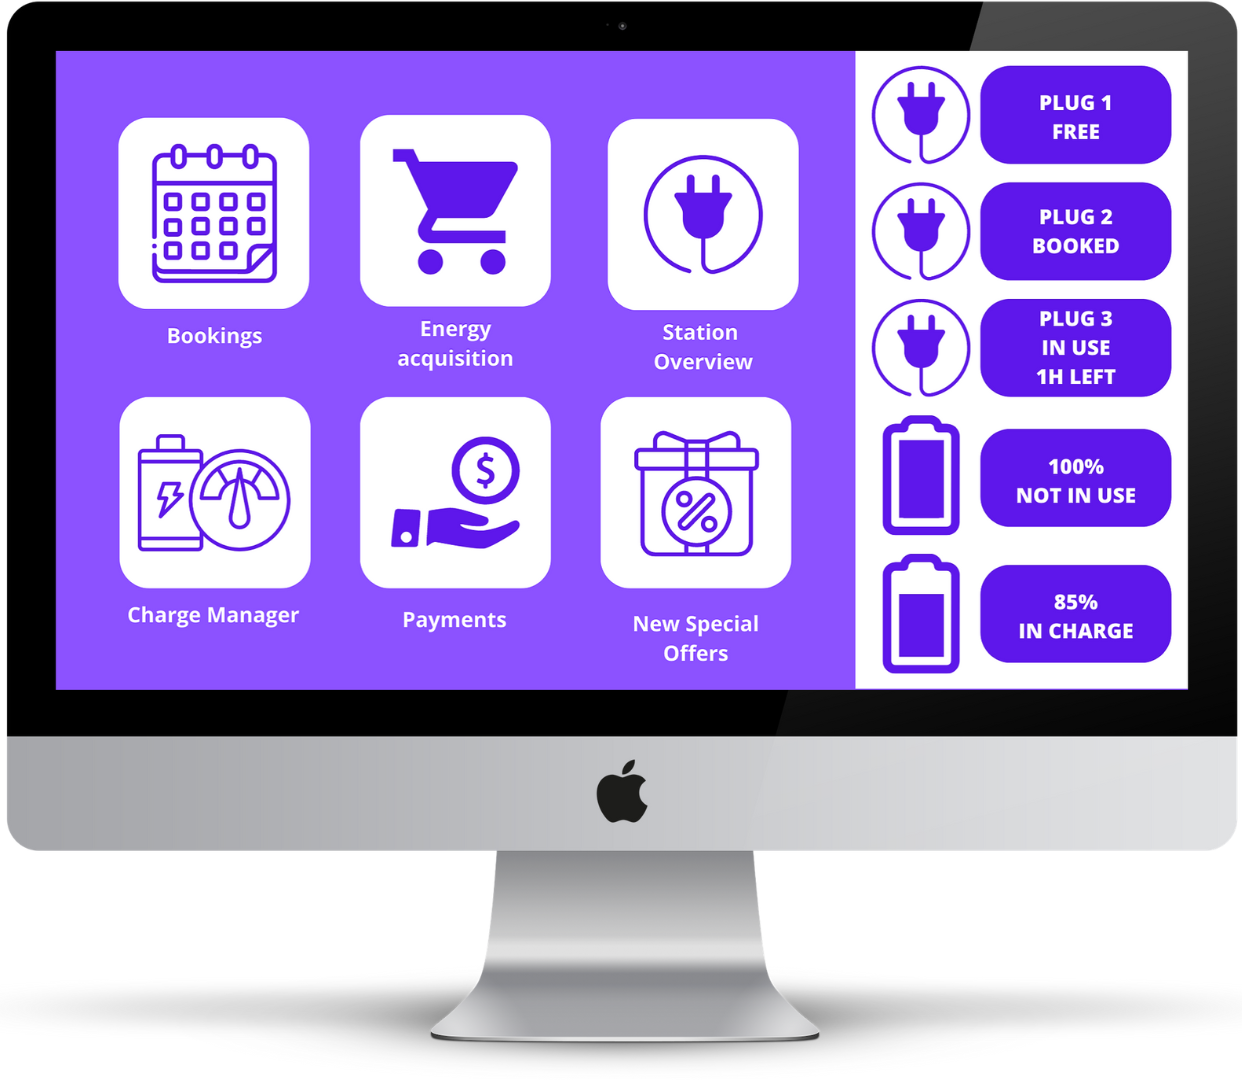
\includegraphics[width = 0.8\textwidth]{assets/cpoi1.png}
        \end{subfigure}
        \begin{subfigure}{0.49\textwidth}
        \centering
        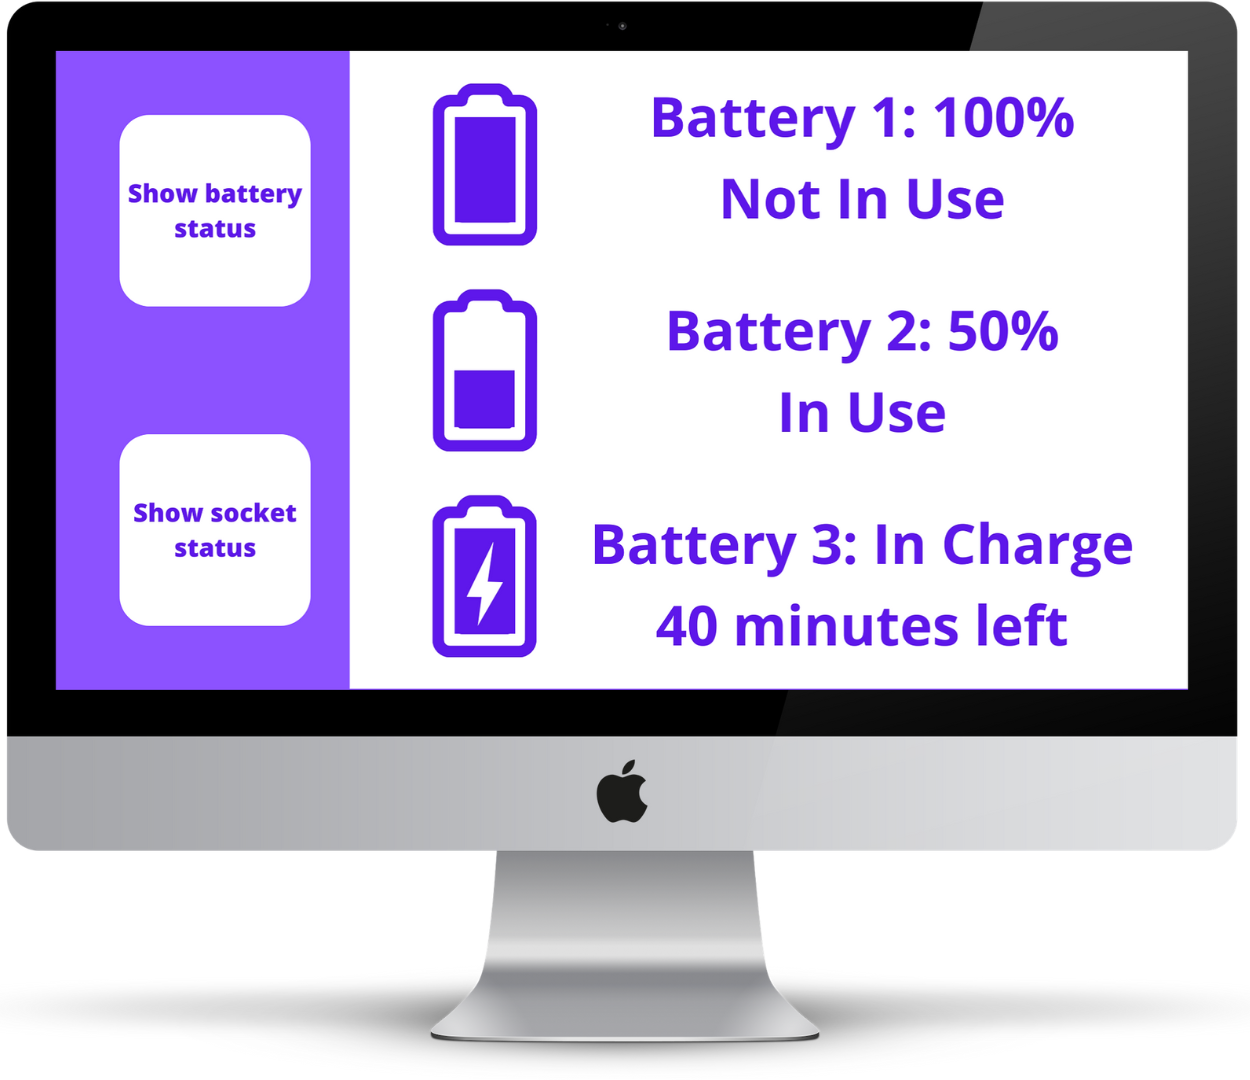
\includegraphics[width = 0.8\textwidth]{assets/cpoi2.png}
        \end{subfigure}
         \begin{subfigure}{0.49\textwidth}
        \centering
        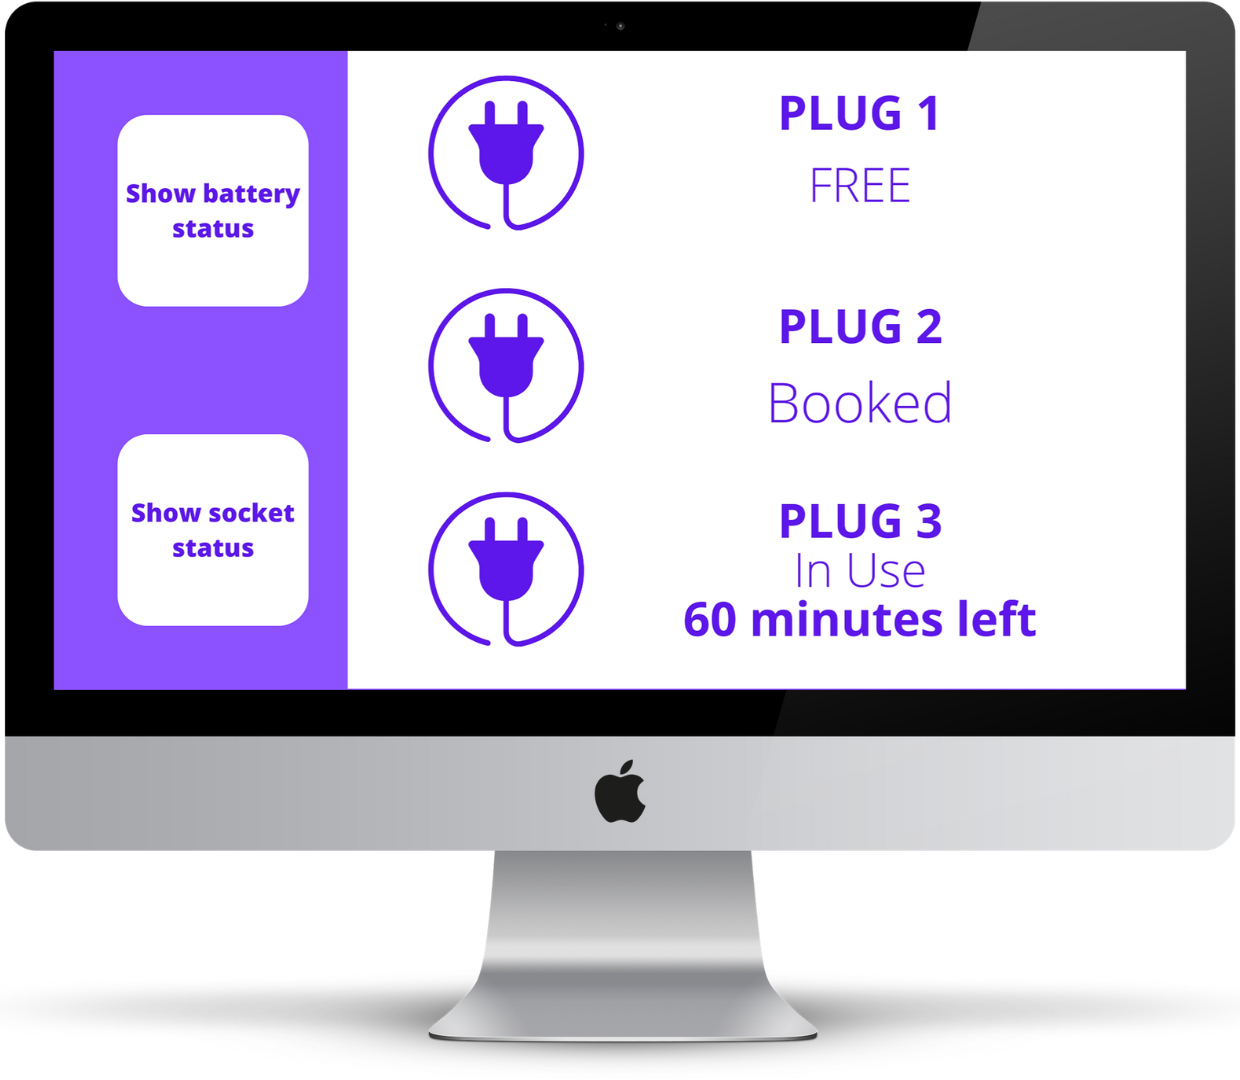
\includegraphics[width = 0.8\textwidth]{assets/cpoi3.png}
        \end{subfigure}
        \begin{subfigure}{0.49\textwidth}
        \centering
        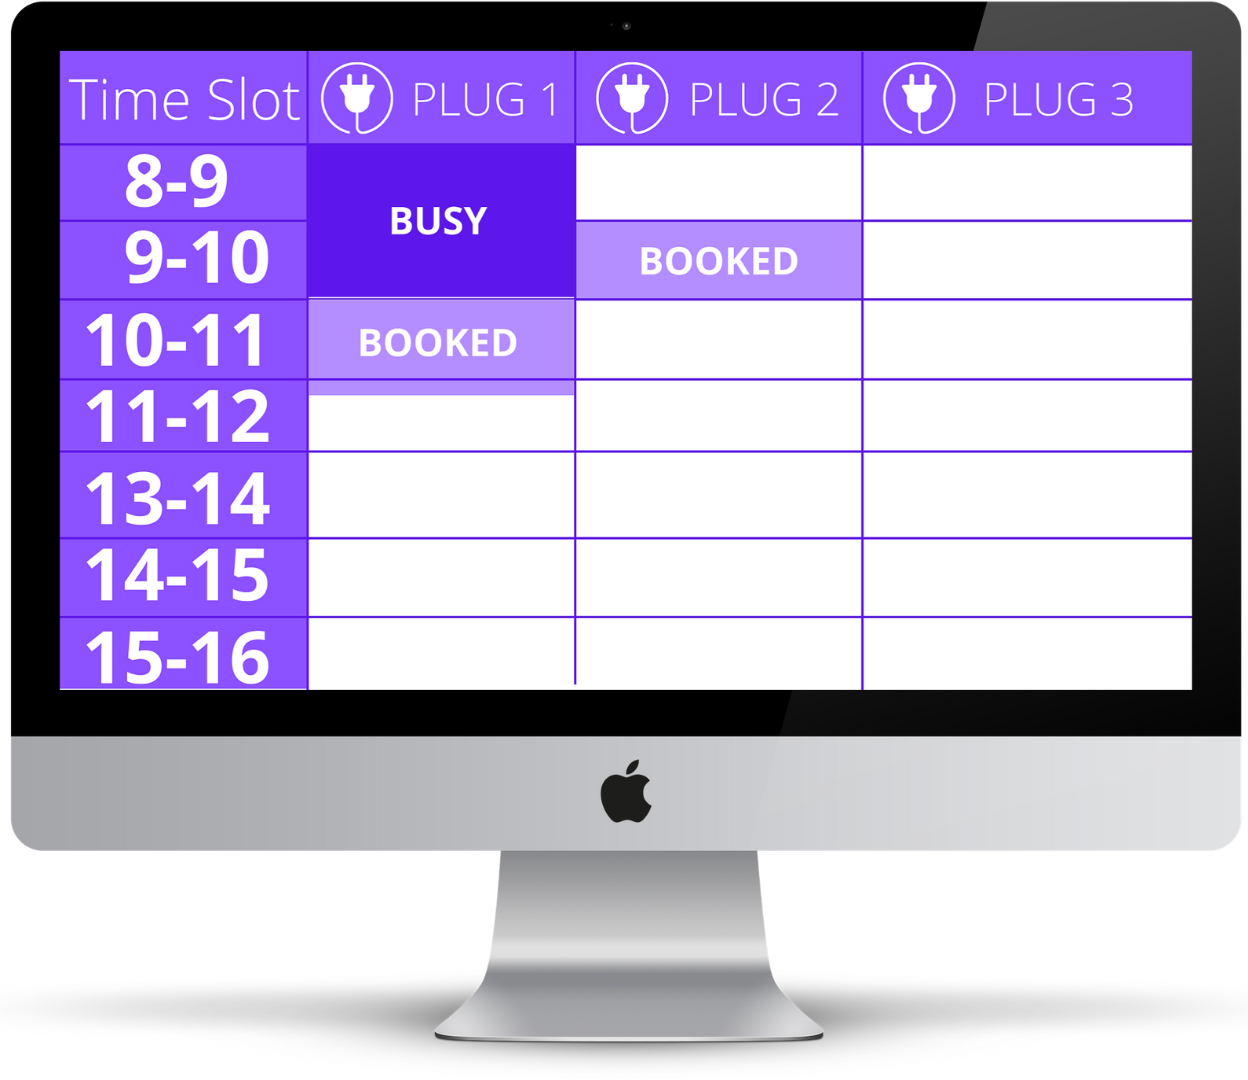
\includegraphics[width = 0.8\textwidth]{assets/cpoi4.png}
        \end{subfigure}
         \begin{subfigure}{0.49\textwidth}
        \centering
        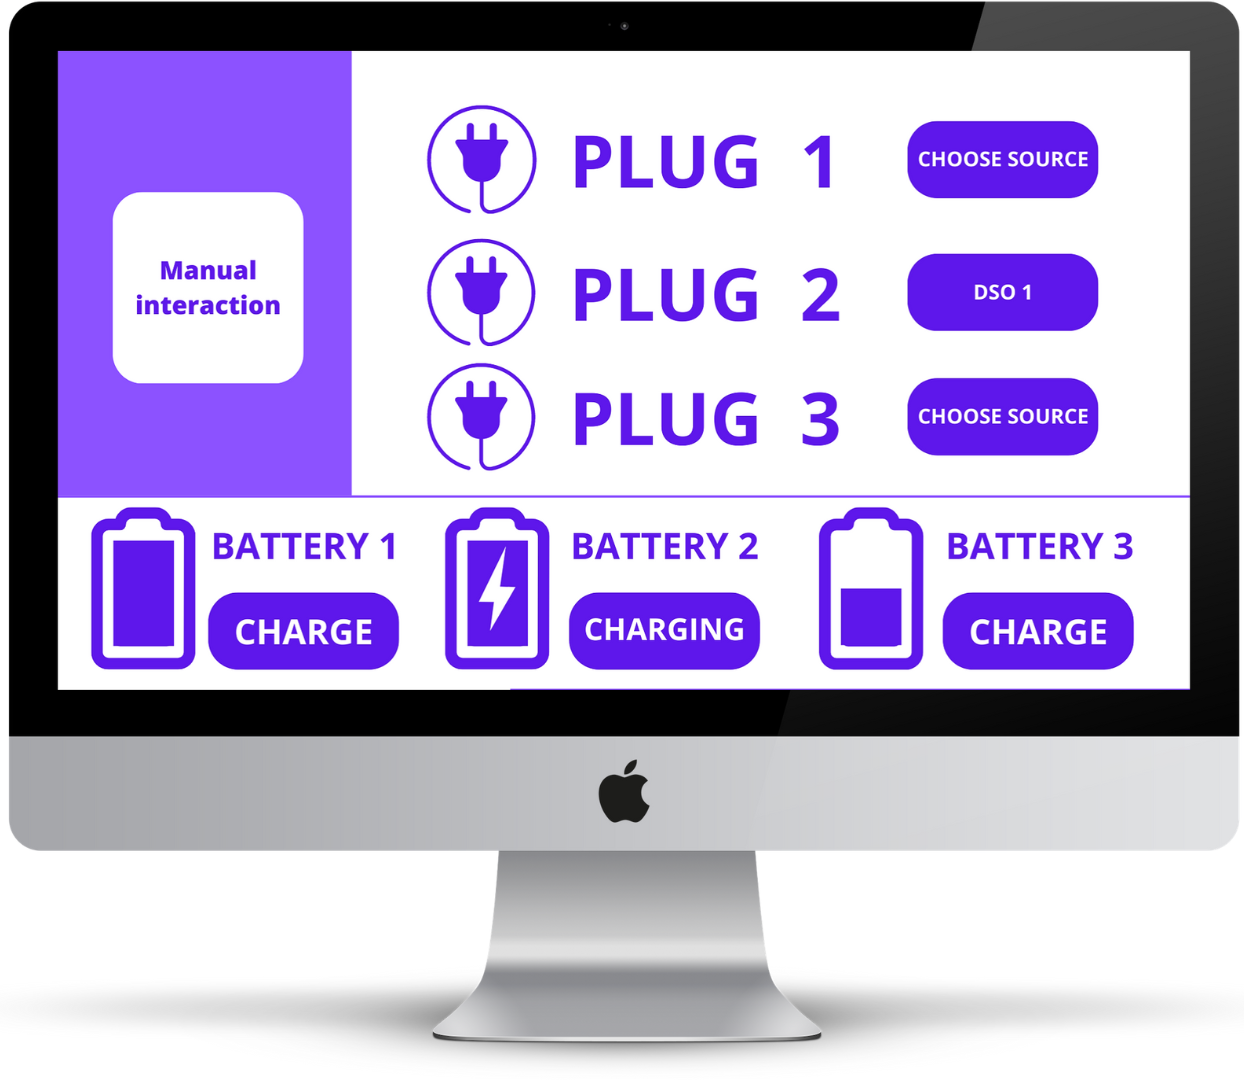
\includegraphics[width = 0.8\textwidth]{assets/cpoi5.png}
        \end{subfigure}
        \begin{subfigure}{0.49\textwidth}
        \centering
        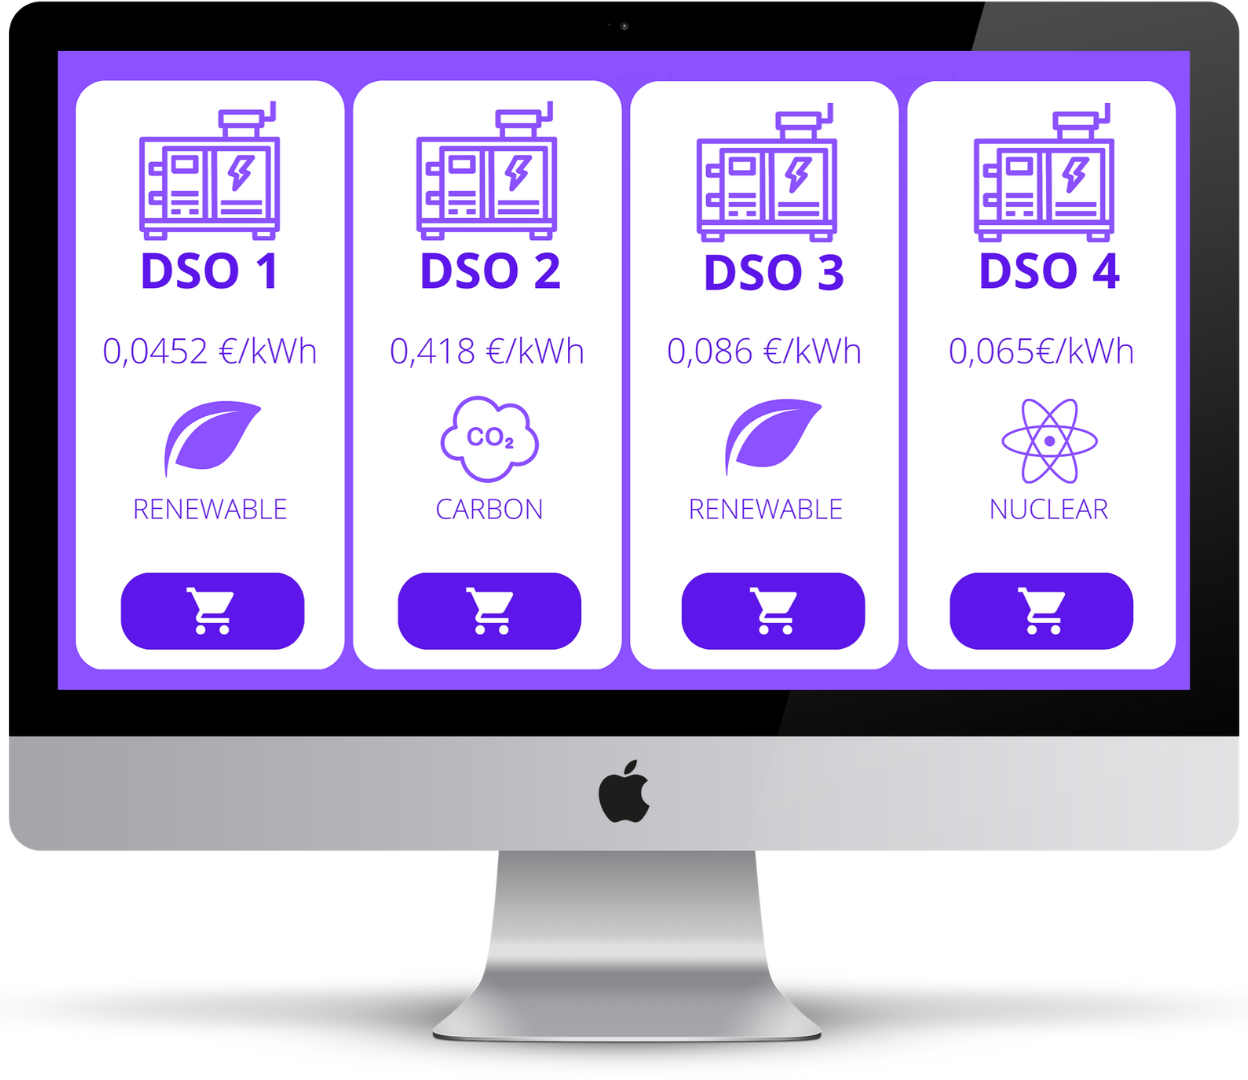
\includegraphics[width = 0.8\textwidth]{assets/cpoi6.png}
        \end{subfigure}
    \caption{CPO interfaces}
    \end{figure}
\clearpage
\chapter{Requirements Traceability}

\section{e-MALL eMSP Goals mapping}
Mapping of goals and related requirements defined in the RASD and associated requirements to the implemented components:

% goal 1
\begin{table}[h]
\begin{tabular}{|
>{\columncolor[HTML]{CBCEFB}}c |l|}
\hline
\cellcolor[HTML]{CBCEFB}                                  & \cellcolor[HTML]{DAE8FC}\begin{tabular}[c]{@{}l@{}}Allow users to know the location, status, prices and special offers provided by\\ charging stations\end{tabular} \\ \cline{2-2} 
\cellcolor[HTML]{CBCEFB}                                  & \cellcolor[HTML]{FFCCC9}\emph{Requirements}: R1, R2, R3, R4, R5, R6, R7, R38, R41, R42                                                                                                                                  \\ \cline{2-2} 
\multirow{-3}{*}{\cellcolor[HTML]{CBCEFB}\textbf{Goal 1}} & \cellcolor[HTML]{ffffff}\emph{eMSP Components}:\\
&- User Dashboard\\
&- User Controller\\
&- Station Info Collector\\
& \emph{CPMS Components}:\\
&- CPO Controller\\
&- Charging Station Manager\\
&-- CollectDataService \\
&-- MonitorChargeService\\
&- CPMS DBMS\\
\hline
\end{tabular}
\caption{Mapping of Goal 1}
\label{tab:my-table1}
\end{table}

% goal 2
\begin{table}[h]
\begin{tabular}{|
>{\columncolor[HTML]{CBCEFB}}c |l|}
\hline
\cellcolor[HTML]{CBCEFB}                                  & \cellcolor[HTML]{DAE8FC}\begin{tabular}[c]{@{}l@{}}Allow users to manage bookings of a charge in a specific location and time\\
frame\end{tabular} \\ \cline{2-2} 
\cellcolor[HTML]{CBCEFB}                                  & \cellcolor[HTML]{FFCCC9}\emph{Requirements}: R1, R2, R8, R9                                                                                                                                      \\ \cline{2-2} 
\multirow{-3}{*}{\cellcolor[HTML]{CBCEFB}\textbf{Goal 2}} & \cellcolor[HTML]{ffffff}\emph{eMSP Components}:\\
&- User Dashboard\\
&- User Controller\\
&- Station Info Collector\\
&- ChargeManager\\
&-- ChargeBookingService\\
&- eMSP DBMS\\
& \emph{CPMS Components}:\\
&- CPO Controller\\
&- Charging Station Manager\\
&-- CollectDataService \\
&-- BookingsManagementService\\
&- CPMS DBMS\\                                                                                                                                      \hline
\end{tabular}
\caption{Mapping of Goal 2}
\label{tab:my-table2}
\end{table}

% goal 3
\begin{table}[h]
\begin{tabular}{|
>{\columncolor[HTML]{CBCEFB}}c |l|}
\hline
\cellcolor[HTML]{CBCEFB}                                  & \cellcolor[HTML]{DAE8FC}\begin{tabular}[c]{@{}l@{}}Allow users to start, monitor and end the charging process {\color[HTML]{DAE8FC}--------------------}
\end{tabular} \\ \cline{2-2} 
\cellcolor[HTML]{CBCEFB}                                  & \cellcolor[HTML]{FFCCC9}\emph{Requirements}: R1, R2, R10, R11, R12, R13, R30, R39                                                                                                                                     \\ \cline{2-2} 
\multirow{-3}{*}{\cellcolor[HTML]{CBCEFB}\textbf{Goal 3}} & \cellcolor[HTML]{ffffff}\emph{eMSP Components}:\\
&- User Dashboard\\
&- User Controller\\
&- Station Info Collector\\
&- ChargeManager\\
&-- Start\&EndService\\
&- eMSP DBMS\\
& \emph{CPMS Components}:\\
&- CPO Controller\\
&- Charging Station Manager\\
&-- CollectDataService \\
&-- Start\&EndService\\
&-- MonitorChargeService\\
&- CPMS DBMS\\                                                                                                                                        \hline
\end{tabular}
\caption{Mapping of Goal 3}
\label{tab:my-table3}
\end{table}

% goal 4
\begin{table}[h]
\begin{tabular}{|
>{\columncolor[HTML]{CBCEFB}}c |l|}
\hline
\cellcolor[HTML]{CBCEFB}                                  & \cellcolor[HTML]{DAE8FC}\begin{tabular}[c]{@{}l@{}}Allow users to pay for the obtained service{\color[HTML]{DAE8FC}------------------------------------------------}\end{tabular} \\ \cline{2-2} 
\cellcolor[HTML]{CBCEFB}                                  & \cellcolor[HTML]{FFCCC9}\emph{Requirements}: R1, R2, R14, R15                                                                                                                                      \\ \cline{2-2} 
\multirow{-3}{*}{\cellcolor[HTML]{CBCEFB}\textbf{Goal 4}} & \cellcolor[HTML]{ffffff}\emph{eMSP Components}:\\
&- User Dashboard\\
&- User Controller\\
&- ChargeManager\\
&-- PaymentService\\
&- eMSP DBMS\\
& \emph{CPMS Components}:\\
&- CPO Controller\\
&- PaymentModule\\
&- CPMS DBMS\\                                       \hline
\end{tabular}
\caption{Mapping of Goal 4}
\label{tab:my-table4}
\end{table}

% goal 5
\begin{table}[h]
\begin{tabular}{|
>{\columncolor[HTML]{CBCEFB}}c |l|}
\hline
\cellcolor[HTML]{CBCEFB}                                  & \cellcolor[HTML]{DAE8FC}\begin{tabular}[c]{@{}l@{}}Suggest users to charge their vehicle based on the charge status, the schedule\\
of the users, special offers provided by the CPOs and availability of the\\charging slots at the identified charging stations\end{tabular} \\ \cline{2-2} 
\cellcolor[HTML]{CBCEFB}                                  & \cellcolor[HTML]{FFCCC9}\emph{Requirements}: R1, R2, R17, R18, R19, R20, R 39, R40                                                                                                                                      \\ \cline{2-2} 
\multirow{-3}{*}{\cellcolor[HTML]{CBCEFB}\textbf{Goal 5}} & \cellcolor[HTML]{ffffff}\emph{eMSP Components}:\\
    &- User Dashboard\\
    &- User Controller\\
    &- Custom Plan Manager\\
    &- Charge Manager\\
    &- eMSP DBMS\\
    & \emph{CPMS Components}:\\
    &- CPO Controller\\
    &- Charging Station Manager\\
    &-- CollectDataService\\
    &-- BookingsManagementService\\
     \hline
\end{tabular}
\caption{Mapping of Goal 5}
\label{tab:my-table5}
\end{table}

\clearpage
\section{e-Mall CPMS Goals mapping}

% goal 6
\begin{table}[h]
\begin{tabular}{|
>{\columncolor[HTML]{CBCEFB}}c |l|}
\hline
\cellcolor[HTML]{CBCEFB}                                  & \cellcolor[HTML]{DAE8FC}\begin{tabular}[c]{@{}l@{}}Provide a complete “external” overview of the charging station (location,\\availability, charging options...){\color[HTML]{DAE8FC}----------------------------------------------------------}\end{tabular} \\ \cline{2-2} 
\cellcolor[HTML]{CBCEFB}                                  & \cellcolor[HTML]{FFCCC9}\emph{Requirements}: R16, R21, R22, R23, R24, R33, R38, R41, R42                                                                                                                                     \\ \cline{2-2} 
\multirow{-3}{*}{\cellcolor[HTML]{CBCEFB}\textbf{Goal 6}} & \cellcolor[HTML]{ffffff}\emph{eMSP Components}:\\
    &- User Dashboard\\
    &- User Controller\\
    &- Station Info Collector\\
    &-- CollectDataService\\
    & \emph{CPMS Components}:\\
    &- CPO Controller\\
    &- Charging Station Manager\\
    &-- CollectDataService\\
    &-- MonitorChargeService\\
    &- CPMS DBMS\\
    \hline
\end{tabular}
\caption{Mapping of Goal 6}
\label{tab:my-table6}
\end{table}

% goal 7
\begin{table}[h]
\begin{tabular}{|
>{\columncolor[HTML]{CBCEFB}}c |l|}
\hline
\cellcolor[HTML]{CBCEFB}                                  & \cellcolor[HTML]{DAE8FC}\begin{tabular}[c]{@{}l@{}}Manage and correctly execute a charge for a specific time frame{\color[HTML]{DAE8FC}---------------}
\end{tabular} \\ \cline{2-2} 
\cellcolor[HTML]{CBCEFB}                                  & \cellcolor[HTML]{FFCCC9}\emph{Requirements}: R16, R21, R22, R23, R24, R25, R26, R27, R28, R29                                                                                                                                      \\ \cline{2-2} 
\multirow{-3}{*}{\cellcolor[HTML]{CBCEFB}\textbf{Goal 7}} & \cellcolor[HTML]{ffffff}\emph{eMSP Components}:\\
    &- User Dashboard\\
    &- User Controller\\
    &- Station Info Collector\\
    &-- CollectDataService\\
    &- eMSP DBMS\\
    & \emph{CPMS Components}:\\
    &- CPO Controller\\
    &- Charging Station Manager\\
    &-- CollectDataService\\
    &-- MonitoeChargeService\\
    &- CPMS DBMS\\                                                                                                                                        \hline
\end{tabular}
\caption{Mapping of Goal 7}
\label{tab:my-table7}
\end{table}

% goal 8
\begin{table}[h]
\begin{tabular}{|
>{\columncolor[HTML]{CBCEFB}}c |l|}
\hline
\cellcolor[HTML]{CBCEFB}                                  & \cellcolor[HTML]{DAE8FC}\begin{tabular}[c]{@{}l@{}}Know the “internal” status of a charging station{\color[HTML]{DAE8FC}-----------------------------------------}\end{tabular} \\ \cline{2-2} 
\cellcolor[HTML]{CBCEFB}                                  & \cellcolor[HTML]{FFCCC9}\emph{Requirements}: R16, R34, R35                                                                                                                                      \\ \cline{2-2} 
\multirow{-3}{*}{\cellcolor[HTML]{CBCEFB}\textbf{Goal 8}} & \cellcolor[HTML]{ffffff}\emph{CPMS Components}:\\
    &- CPO Dashboard\\
    &- CPO Controller\\
    &- Battery Management Module\\
    &-- CollectBatteryPercentageService\\
    &- Charging Station Manager\\
    &-- CollectDataService\\
    &-- MonitorChargeService\\
    &- CPMS DBMS\\                                                                                                                                       \hline
\end{tabular}
\caption{Mapping of Goal 8}
\label{tab:my-table8}
\end{table}
\clearpage
% goal 9
\begin{table}[h]
\begin{tabular}{|
>{\columncolor[HTML]{CBCEFB}}c |l|}
\hline
\cellcolor[HTML]{CBCEFB}                                  & \cellcolor[HTML]{DAE8FC}\begin{tabular}[c]{@{}l@{}}Handle the payment of a charge{\color[HTML]{DAE8FC}-------------------------------------------------------------}\end{tabular} \\ \cline{2-2} 
\cellcolor[HTML]{CBCEFB}                                  & \cellcolor[HTML]{FFCCC9}\emph{Requirements}: R16, R30, R31                                                                                                                                      \\ \cline{2-2} 
\multirow{-3}{*}{\cellcolor[HTML]{CBCEFB}\textbf{Goal 9}} & \cellcolor[HTML]{ffffff}\emph{CPMSComponents}:\\
    &- CPO Controller\\
    &- Payment Module\\
    &-- PaymentService\\
    &- CPMS DBMS\\                                                                                                                                        \hline
\end{tabular}
\caption{Mapping of Goal 9}
\label{tab:my-table9}
\end{table}
\bigskip

% goal 10
\begin{table}[h]
\begin{tabular}{|
>{\columncolor[HTML]{CBCEFB}}c |l|}
\hline
\cellcolor[HTML]{CBCEFB}                                  & \cellcolor[HTML]{DAE8FC}\begin{tabular}[c]{@{}l@{}}Provide the eMSP with the most convenient charging options by choosing to\\use locally stored energy or acquire it from DSOs
\end{tabular} \\ \cline{2-2} 
\cellcolor[HTML]{CBCEFB}                                  & \cellcolor[HTML]{FFCCC9}\emph{Requirements}: R16, R32, R36, R37                                                                                                                                      \\ \cline{2-2} 
\multirow{-3}{*}{\cellcolor[HTML]{CBCEFB}\textbf{Goal 10}} & \cellcolor[HTML]{ffffff}\emph{CPMS Components}:\\
    &- CPO dashboard\\
    &- CPO Controller\\
    &- Battery Management Module\\
    &-- SwitchCharginSourceService\\
    &- DSO Info Collector\\
    &-- CollectDataService\\
    &- CPMS DBMS\\                                                                                                                                        \hline
\end{tabular}
\caption{Mapping of Goal 10}
\label{tab:my-table10}
\end{table}
\clearpage

\chapter{Implementation, Integration and Test Plan}
This section contains a description of the implementation plan and the order in which the subcomponents will be implemented and integrated. It also contains a plan for system testing.

\section{Implementation plan}
As discussed previously and in the RASD, e-MALL is a complex system consisting of \emph{two communicating subsystems}, which proved to be a challenge during development. For this reason, e-MALL CPMS and eMSP were designed as two almost separate software components whose interaction should be as platform independent as possible. This was also considered a requirement, as e-MALL eMSP should interact seamlessly with third-party CPMS, so designing them as independently as possible seemed as the most optimal approach.\\

\noindent A bottom-up approach was used to implement each system. In a bottom-up approach, the entire system can be built incrementally by developing each component independently and gradually integrating it into the overall system. Each component can be tested separately before being integrated into the system to prevent the occurrence of errors as early as possible.\\

\bigskip
\subsubsection{e-MALL eMSP implementation}
The first services to be implemented are the storage ones, so the setup of a DB and DBMS, and the development of the interfaces between the system and the databases.\newline
The eMSP sub-system is made of three main components:
\begin{enumerate}
    \item\textbf{Charge manager}: Used to store user related data in the DB. Also interacts with external banking APIs to provide a payment platform.\newline
    User wise, it provides all the tools to start, end and book a charge.    
    \item\textbf{Custom plan manager}: Used to create an \emph{user-tailored} charging plan via data mining, as well as proactively suggest charging options.
    \item\textbf{Station info collector}: Used to connect to Google Maps' APIs and CPMS in order to provide a complete representation of the stations along with the corresponding special offers.
\end{enumerate}

\noindent The first modules to be implemented and tested were [1] and [3]. This allowed to test and debug an almost working system. Module [2] is defined as an \emph{advanced feature} of e-MALL, which was considered an "optional" during the development phase, being completely independent from the other services; as well as not having any side-effect on the system.\newline
Each service has been developed from scratch and initially provides all the methods for communicating with DBMS and performing all the necessary queries to store and retrieve data.\newline
The next step was the development of the \emph{User Controller}, which acts as a translation layer between the data processing modules and the \emph{User Interface}. It is the module responsible for executing all service calls based on the user input.\newline
Last but not least, we designed the \emph{User Dashboard}, a graphical user interface designed to be as simple and engaging as possible.\\

\bigskip
\subsubsection{e-MALL CPMS implementation}
As mentioned earlier, the priority was to set up DB and DBMS to enable data storage and retrieval. After that, the main components were designed:
\begin{enumerate}
    \item\textbf{Payment module}: Used to manage payments provided by users and is connected to banking APIs.
    \item\textbf{Battery management module}: Used to manage local batteries. They can be recharged during a charging operation or provide additional charge when needed.
    \item\textbf{Charging station manager}: Used to provide a complete overview of the charging station by displaying available, booked or free outlets, and local batteries status (if available). Also allows for manual interaction during a charge.
    \item\textbf{DSO info collector}: Used for communication with DSOs and power procurement.
\end{enumerate}

\noindent As stated in the RASD, manual intervention by an operator is supported because the CPO must be able to manage his own charging station. However, this aspect was only implemented in the final stages of development, as testing and debugging a complete and autonomous implementation was key to making the system manually usable later.\newline
The first component to be implemented was [3], it enables the most important functions of the CPMS, therefore its correct implementation would eliminate the major bugs and vulnerabilities. The choice of the next component to implement was [2], in order to easily manage the whole station correctly. [1] and [4] were then implemented in parallel, as they both rely on external interfaces and don't interact with other modules for state-changing tasks.\newline
The next component to be implemented was the \emph{CPMS controller} and finally CPO's GUI (also called \emph{CPO dashboard}).\newline
A similar approach as stated in the eMSP section was used, first all services that perform data queries were designed, using, as always, a \emph{bottom-up} approach.\newline
Lastly, the interaction between the system and external APIs is tested.


\section{Integration plan}
The following diagrams represent the integration of the various components. The diagrams are ordered by the priority with which they are to be implemented, as indicated in the previous section.\\
The integration was split into \emph{levels}. Each level follows the \emph{bottom up} approach.\newline
Despite different components, the subsystems are structured similarly, so the integration strategy is the same.\\
All components are implemented and tested by a \emph{Mock object} that emulates the components not yet implemented.

\subsection{eMSP integration plan}

\subsubsection{Level 0}
The first component to be implemented is the DBMS Service, essential for all the other components.

\bigskip
\begin{figure}[ht]
    \centering
    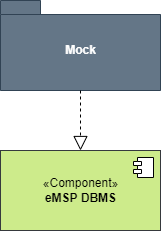
\includegraphics[width=0.2\textwidth]{assets/level0_emsp_integration.png}
    \caption{\textbf{Level 0}: integration of the eMSP DBMS services}
    \label{fig:my_label4323323}
\end{figure}
\clearpage

\subsubsection{Level 1}
After the DBMS services are implemented, all components that interact with them can be integrated and tested. The StationInfoCollector module can also be developed in parallel, since it does not interact with DBMS, but is integrated later.

\bigskip
\begin{figure}[ht]
    \centering
    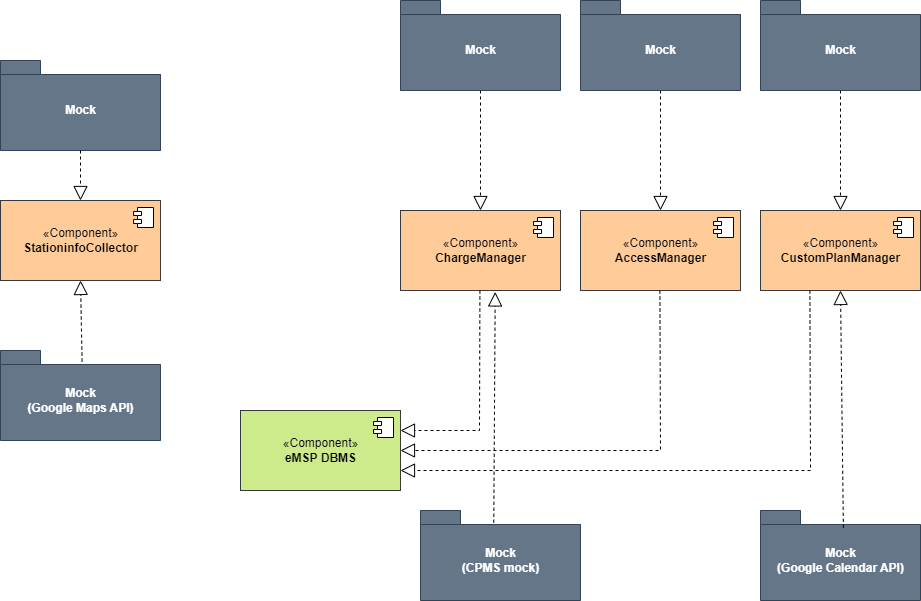
\includegraphics[width=\textwidth]{assets/level1_emsp_integration.png}
    \caption{\textbf{Level 1}: integration of the main eMSP services}
    \label{fig:my_label40}
\end{figure}
\clearpage

\subsubsection{Level 2}
Now that the main services have been tested and integrated, the UserController, which is responsible for calling the main services, can be tested and integrated.

\bigskip
\begin{figure}[ht]
    \centering
    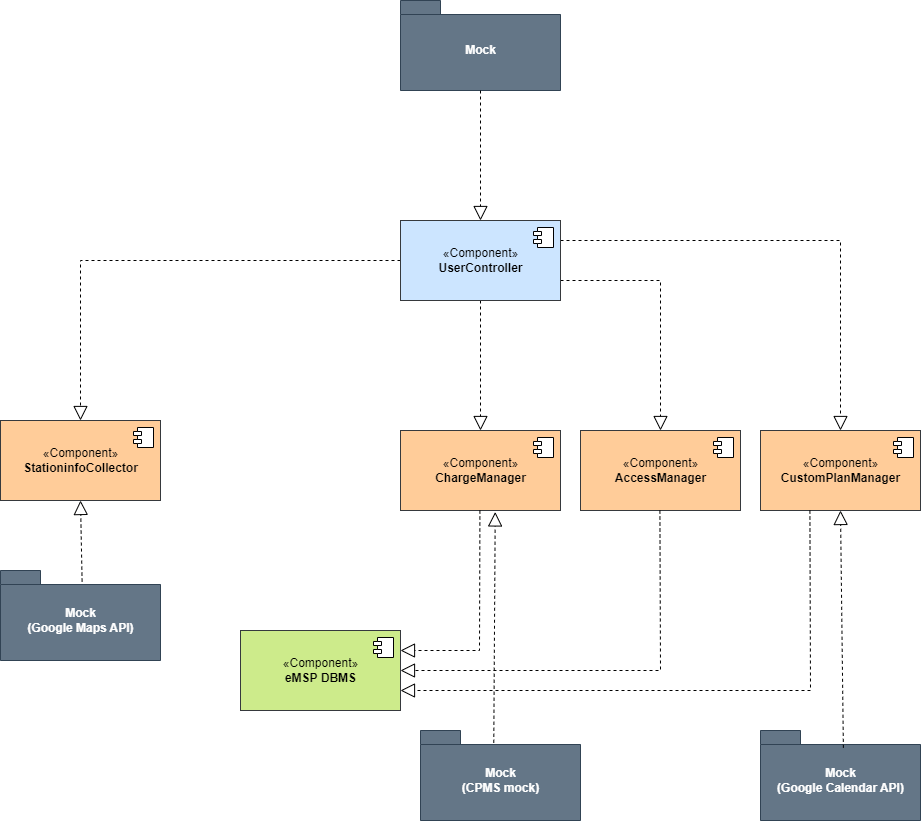
\includegraphics[width=\textwidth]{assets/level2_emsp_integration.png}
    \caption{\textbf{Level 2}: integration of the UserController}
    \label{fig:my_label42333333}
\end{figure}
\clearpage

\subsubsection{Level 3}
Now that the UserController has been tested and integrated, the UserDashboard, which is responsible for receiving the user inputs, can be tested and integrated.

\bigskip
\begin{figure}[ht]
    \centering
    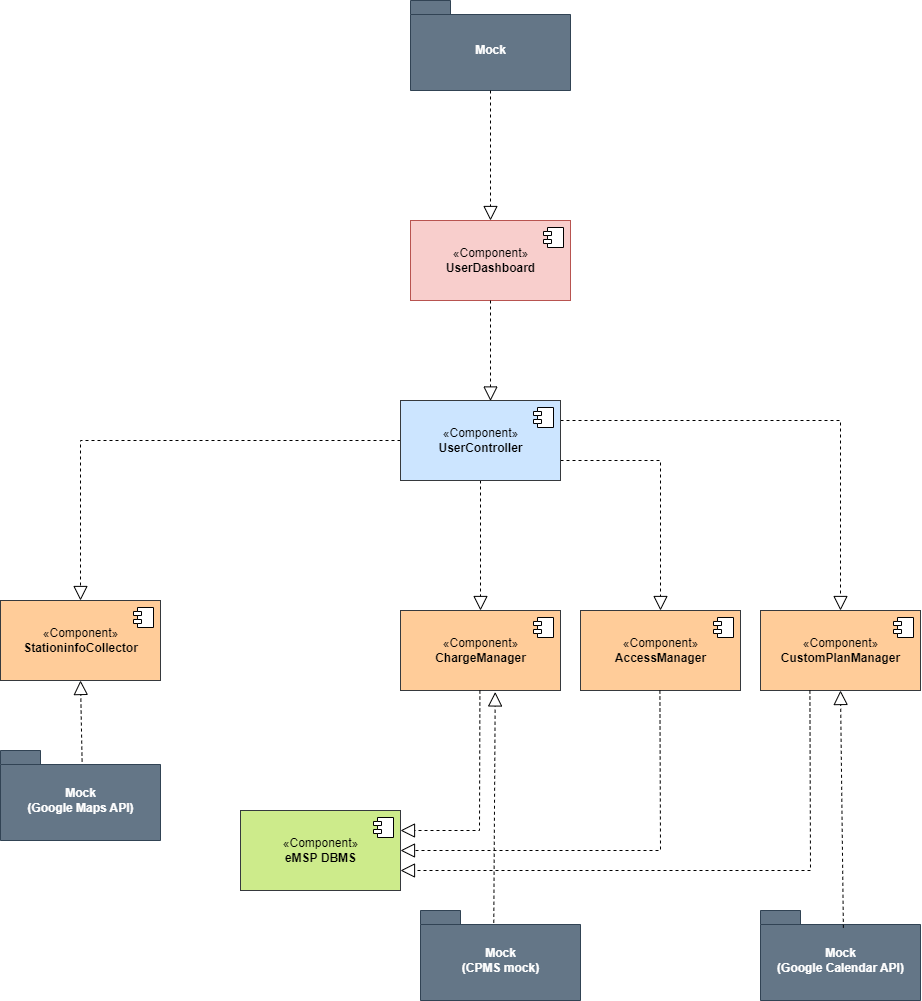
\includegraphics[width=0.9\textwidth]{assets/level3_emsp_integration.png}
    \caption{\textbf{Level 3}: integration of the UserDashboard}
    \label{fig:my_label423331333}
\end{figure}
\clearpage


\subsection{CPMS integration plan}

\subsubsection{Level 0}
The first component to be implemented is the DBMS Service, essential for all the other components.

\bigskip
\begin{figure}[ht]
    \centering
    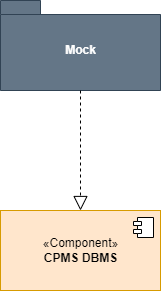
\includegraphics[width=0.2\textwidth]{assets/level0_CPMS_integration.png}
    \caption{\textbf{Level 3}: integration of the CPMS DBMS Services}
    \label{fig:my_label423377731333}
\end{figure}
\clearpage

\subsubsection{Level 1}
After the DBMS services are implemented, all components that interact with them can be integrated and tested.

\bigskip
\begin{figure}[ht]
    \centering
    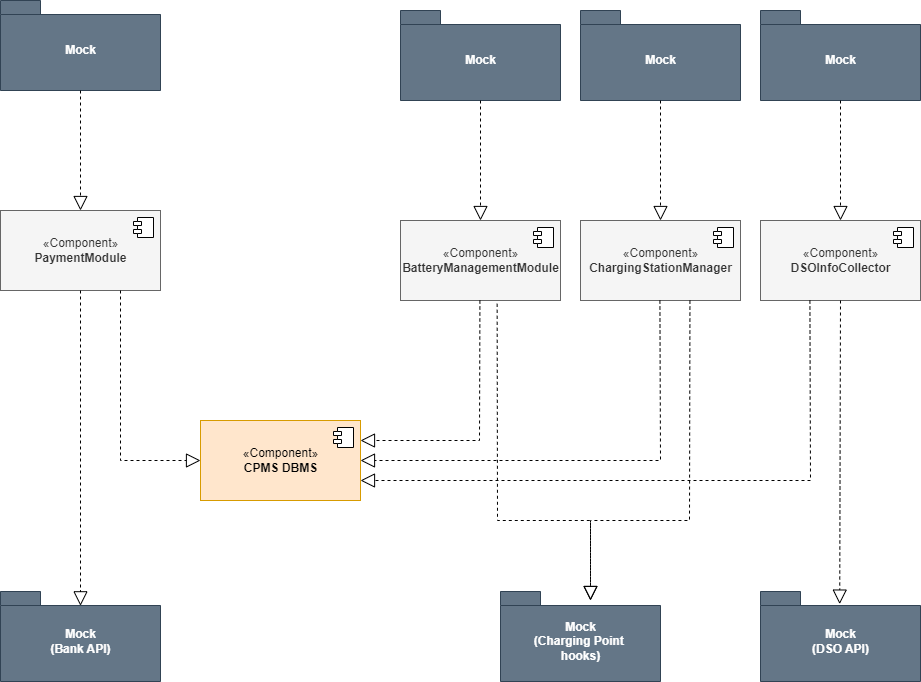
\includegraphics[width=\textwidth]{assets/level1_CPMS_integration.png}
    \caption{\textbf{Level 1}: integration of the main services}
    \label{fig:my_label423666331333}
\end{figure}
\clearpage

\subsubsection{Level 2}
Now that the main services have been tested and integrated, the CPOController, which is responsible for calling the main CPMS services, can be tested and integrated.

\bigskip
\begin{figure}[ht]
    \centering
    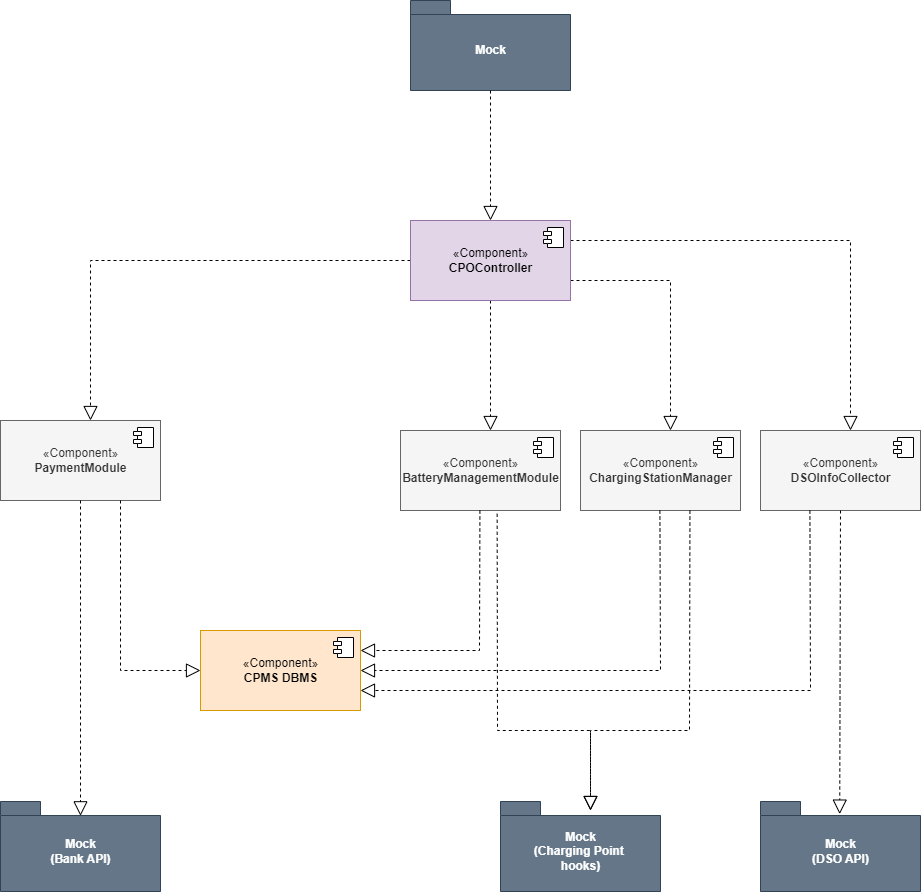
\includegraphics[width=\textwidth]{assets/level2_CPMS_integration.png}
    \caption{\textbf{Level 2}: integration of the CPOController}
    \label{fig:my_label42366633133223}
\end{figure}
\clearpage

\subsubsection{Level 3}
Now that the CPOController has been tested and integrated, the CPODashboard, which is responsible for receiving the CPO inputs, can be tested and integrated.

\bigskip
\begin{figure}[ht]
    \centering
    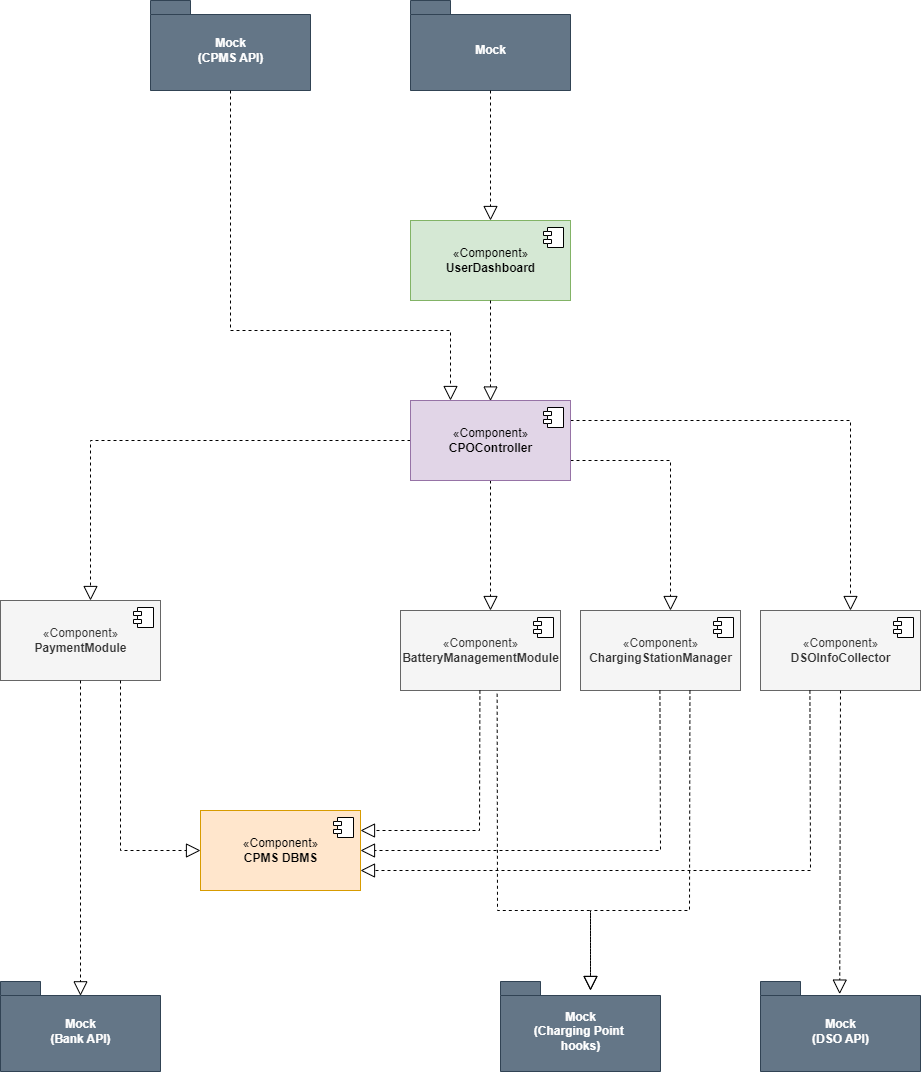
\includegraphics[width=0.9\textwidth]{assets/level3_CPMS_integration.png}
    \caption{\textbf{Level 3}: integration of the CPODashboard}
    \label{fig:my_label42366434343436331333}
\end{figure}
\clearpage

\subsection{Subsystems integration plan}
Now that all components of the two subsystems have been tested and integrated, they can be integrated again to test the communication between them.\\
The API calls are still present, as they will be removed once the communication has been thoroughly tested.

\bigskip
\begin{figure}[ht]
    \centering
    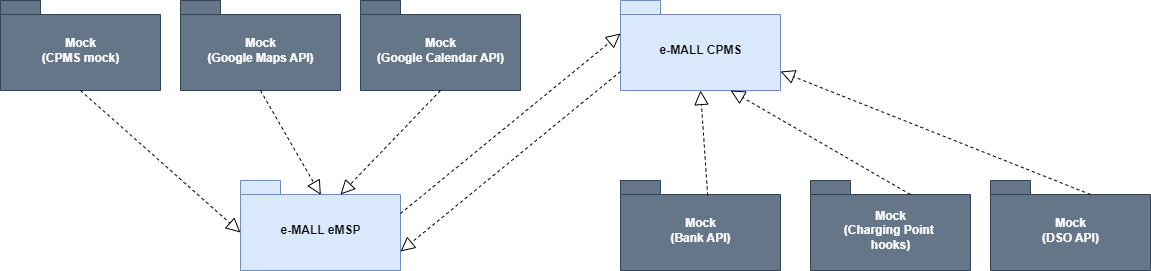
\includegraphics[width=1.1\textwidth]{assets/high_level_integration.png}
    \caption{Integration of the two subsystems}
    \label{fig:my_label4236643411143436331333}
\end{figure}
\clearpage

\section{System testing}
Unit tests are the first step. Each implemented class must work as intended, including covering all possible corner cases.\\
The next step is integration testing with increasing levels of aggregation, ensuring that communication and data exchange work as intended.\\
The main goal of testing is to guarantee that all promised features work, so extensive testing is performed on all features.\\
All testing is done with a \emph{bottom up} approach, meaning every small class is thoroughly tested before implementation.\\
A special effort is also made to guarantee \emph{non-functional} requirements:
\begin{itemize}
    \item\textbf{Performance testing}: testing speed, scalability, stability and reliability of the system
    \item\textbf{Load testing}: testing the behavior of the system under high loads
    \item\textbf{Stress testing}: testing the robustness of the system under
    varying loads and intensity
\end{itemize}

\chapter{Effort Spent}

\section{Effort required by members}
\begin{table}[h]
\centering
\begin{tabular}{|l|c|}
\hline
\multicolumn{1}{|c|}{Task}      & Time \\ \hline
Introduction                    & 2h    \\ \hline
High-Level Component view       & 2h    \\ \hline
Deployment view                 & 3h    \\ \hline
Requirements traceability       & 2h    \\ \hline
Implementation, Integration and Test Plan     & 3h    \\ \hline
Rewriting and general fixes & 4h \\ \hline
Final review & 4h \\ \hline
\end{tabular}
\caption{Marco Lorenzo Campo}
\label{tab:my-table11}
\end{table}

\begin{table}[h]
\centering
\begin{tabular}{|l|c|}
\hline
\multicolumn{1}{|c|}{Task}      & Time \\ \hline
Introduction                    & 2h    \\ \hline
High-Level Component view       & 2h    \\ \hline
Runtime view                    & 6h    \\ \hline
Component Interfaces            & 5h    \\ \hline
Rewriting and general fixes & 3h \\ \hline
Final review & 2h \\ \hline
\end{tabular}
\caption{Alessia Abbondanza}
\label{tab:my-table15}
\end{table}

\begin{table}[h]
\centering
\begin{tabular}{|l|c|}
\hline
\multicolumn{1}{|c|}{Task}      & Time \\ \hline
Introduction                    & 2h    \\ \hline
 Component view       & 3h    \\ 
 \hline
Component Interfaces            & 3h    \\ \hline
User Interface Design            & 4h    \\ \hline
Requirements traceability       & 2h    \\ \hline
Implementation, Integration and Test Plan     & 3h    \\ \hline
Rewriting and general fixes & 1h \\ \hline
Final review & 2h \\ \hline
\end{tabular}
\caption{Alessandro De Luca}
\label{tab:my-table14}
\end{table}

\chapter{RASD references}
Here's a summary of goals and requirements provided in the RASD:\\

\section{eMSP Goals}
\begin{itemize}
    \item[\textbf{G1.}]   Allow users to know the location, status, prices and special offers provided by charging stations
    \item[\textbf{G2.}]  Allow users to manage bookings of  a charge in a specific location and time frame
    \item[\textbf{G3.}] Allow users to start, monitor and end the charging process
    \item[\textbf{G4.}] Allow users to pay for the obtained service
    \item[\textbf{G5.}] Suggest users to charge their vehicle based on the charge status, the schedule of the users, special offers provided by the CPOs and availability of the charging slots at the identified charging stations\\
\end{itemize}

\section{CPMS Goals}
\begin{itemize}
    \item[\textbf{G6.}] Provide a complete “external” overview of the charging station (location, availability, charging options…)
    \item[\textbf{G7.}] Manage and correctly execute a charge for a specific time frame
    \item[\textbf{G8.}] Know the “internal” status of a charging station
    \item[\textbf{G9.}] Handle the payment of a charge
    \item[\textbf{G10.}] Provide the eMSP with the most convenient charging options by choosing to use locally stored energy or acquire it from DSOs
\end{itemize}

\section{Requirements}
\begin{itemize}
    \item[\textbf{R1.}]The e-MALL application should allow users to register by providing their email address
    
    \item[\textbf{R2.}]The e-MALL application should allow users to login using the credentials input at registration time
    
    \item[\textbf{R3.}]The e-MALL application should retrieve locations of charging stations from their CPMS
    
    \item[\textbf{R4.}]The e-MALL application should show availability of charging stations from their CPMS
    
    \item[\textbf{R5.}]The e-MALL application should retrieve prices of charging stations from their CPMS
    
    \item[\textbf{R6.}]The e-MALL application should retrieve special offers of charging stations from their CPMS
    
    \item[\textbf{R7.}]The e-MALL application should acquire locations of charging stations from their CPMS
    
    \item[\textbf{R8.}]The e-MALL application should allow the user to book a charging station for a specific location and time frame
    
    \item[\textbf{R9.}]The e-MALL application should allow the user to delete a previously booked charging station
    
    \item[\textbf{R10.}]The e-MALL application should register a start signal when the “start charge” button is pressed
    
    \item[\textbf{R11.}]The e-MALL application should forward the start signal of the charging to the CPMS 
    
    \item[\textbf{R12.}]The e-MALL application should register an end signal when the “end charge” button is pressed
    
    \item[\textbf{R13.}]The e-MALL application should forward the end signal of the charging to the CPMS
    
    \item[\textbf{R14.}]The e-MALL application should allow users to insert their banking credentials
    
    \item[\textbf{R15.}]The e-MALL application should be able to communicate with the user’s bank
    
    \item[\textbf{R16.}]The e-MALL application should connect to external CPMSs through API
    
    \item[\textbf{R17.}]The e-MALL application should know the charge status of the user’s vehicle
    
    \item[\textbf{R18.}]The e-MALL application should know the daily schedule of the user
    
    \item[\textbf{R19.}]The e-MALL application should be aware of special offers provided by the CPO
    
    \item[\textbf{R20.}]The e-MALL application should be aware of the availability of charging slots at the identified station
    
    \item[\textbf{R21.}]The CPMS should collect real time information about available charging sockets
    
    \item[\textbf{R22.}]The CPMS should collect real time information about the charge speed provided by each charging socket (classified as slow, fast or rapid)
    
    \item[\textbf{R23.}]The CPMS should collect real time information about the cost of a charge
    
    \item[\textbf{R24.}]The CPMS should collect real time information about the estimated time to completion of a charge currently happening
    
    \item[\textbf{R25.}]The CPMS should set an “available” socket as “unavailable” for 15 minutes after it receives a booking
    
    \item[\textbf{R26.}]The CPMS should set a booked socket as “available” if no charge has been started for 15 minutes
    
    \item[\textbf{R27.}]The CPMS should set a booked socket as “available” if the eMSP deletes the relative booking
    
    \item[\textbf{R28.}]The CPMS should set a socket as “unavailable” as long as a charge is in process
    
    \item[\textbf{R29.}]The CPMS should stop dispensing power when the plugged battery is fully charged
    
    \item[\textbf{R30.}]The CPMS should provide real time expenses of a charge
    
    \item[\textbf{R31.}]The CPMS should receive payments from the eMSP
    
    \item[\textbf{R32.}]The CPMS should communicate with DSOs’ API to retrieve the cost of energy
    
    \item[\textbf{R33.}]The CPMS should choose the most convenient DSO based on the eMSPs’ charge requests
    
    \item[\textbf{R34.}]The CPMS should know the CPOs’ local energy availability 
    
    \item[\textbf{R35.}]The CPMS should know if batteries are available in the charging station
    
    \item[\textbf{R36.}]The CPMS should compute where to dispense energy from (local batteries, DSOs or a mixture of the two), to provide the most convenient options
    
    \item[\textbf{R37.}]The CPMS should allow operators to manually handle the energy acquisition and dispense procedure
    
    \item[\textbf{R38.}]The CPMS should communicate the current special offers to the e-MALL application
    
    \item[\textbf{R39.}]The e-MALL application should know the charge status of the user’s vehicle
    
    \item[\textbf{R40.}]The e-MALL application should know the daily schedule of the user
    
    \item[\textbf{R41.}]The e-MALL application should be aware of special offers provided by the CPO
    
    \item[\textbf{R42.}]The e-MALL application should be aware of the availability of charging slots at the identified station
\end{itemize}


\chapter{References}
\begin{itemize}
    \item J2EE Web Servers Load Balancing.
    \item William Stallings and Lawrie Brown. Computer Security: Principles and Practice. Prentice Hall Press, USA, 3rd edition, 2014.
    \item Ingegneria del software. Binato, A., Fuggetta, A. and Sfardini, L., 2006. Milano: Pearson education Italia.
    \item Link: Relational vs. Non-Relational Database: Pros \& Cons | The Aloa Blog, accessed: 2022-01-09, Aloa Blog, Pawlan David.
    \item What is HTTPS? | Cloudflare.
    \item MDN Web Docs Glossary: Definitions of Web-related terms - MVC
    \item OCPI 2.2: Open Charge Point Interface -document version 2.2-d2, 12-06-2020
    \item Setting The Standard: OCPP 1.6 vs 2.0.1 - Noah Newfield, October 22, 2020
\end{itemize}  

\end{document}
